% !TeX program = xelatex
% !TeX encoding = UTF-8
\documentclass{MathorCupmodeling}
\usepackage{amsmath,amssymb}
\usepackage{array}
\usepackage{booktabs}
\usepackage{calc}
\usepackage{enumitem}
\usepackage{float}
\usepackage{graphicx}
\usepackage{hyperref}
\usepackage{longtable}
\usepackage{placeins}
\usepackage{tabularx}
\graphicspath{{figures/}{src/outputs/figures/}}

% ---- 浮动体排版参数：为大图留出更宽松的顶/底放置空间 ----
\renewcommand{\topfraction}{0.9}
\renewcommand{\bottomfraction}{0.8}
\renewcommand{\textfraction}{0.1}
\renewcommand{\floatpagefraction}{0.75}
\setcounter{topnumber}{3}
\setcounter{bottomnumber}{2}
\setcounter{totalnumber}{4}

\setlist[enumerate]{nosep,leftmargin=2em}
\renewcommand{\arraystretch}{1.15}
\providecommand{\tightlist}{%
  \setlength{\itemsep}{0pt}\setlength{\parskip}{0pt}}
\newcommand{\pandocbounded}[1]{#1}

\bianhao{MC2606970}
\tihao{C}
\timu{中老年人群高血脂症的风险预警及干预方案优化}
\keyword{中老年高血脂症；中医体质辨识；痰湿体质；多重共线性；Borda 排序聚合；双轴可解释评分卡；Apriori 关联规则；动态规划}

\begin{document}

\begin{abstract}
针对中老年人群高血脂症高发的公共卫生问题，本文融合中医体质类型分类、痰湿体质特征量化、中老年人活动量表评分及血常规体检数据，构建了``\textbf{数据清洗---关键指标筛选---三级风险预警---六个月个性化干预优化}''的多维度数学建模方案。

\textbf{数据清洗}：对 1000 例样本进行系统性质量检查，确认无缺失值与重复 ID，ADL/IADL 子项之和与总分完全吻合；检出 \textbf{65 例（6.5\%）体质标签与最高积分体质不一致}的判定歧义样本，标注保留；利用 Tukey IQR 准则发现各血脂指标仅 0\%--1.4\% 的离群值，多为真实病理表现，不作删除。本文还验证了\textbf{诊断标签与 ``血脂异常项数 $\ge 1$'' 一致率为 100\%}，揭示出血脂指标天然具有信息泄漏风险，这一发现直接指导了问题二的模型选型。

\textbf{问题一}：将候选特征限定为\textbf{血常规指标（7 项）+ 活动量表评分（ADL/IADL 子项 10 项）}，共 17 个指标。先进行\textbf{多重共线性诊断（VIF）}剔除 $\text{ADL总分}=\Sigma \text{ADL}_i$ 这类完全共线的汇总项，再采用 5 种互补方法\textbf{（Spearman 秩相关、互信息、弹性网络回归、随机森林置换重要度、偏相关）}；方法选取遵循``参数／非参数 $\times$ 线性／非线性 $\times$ 单变量／控制其它变量''的三维正交覆盖原则。采用 \textbf{Borda 排序聚合}作为综合排序方法,规避量纲与分布偏态带来的偏差。结果：表征痰湿体质严重程度最优 Top-5 指标依次为 \textbf{TC、ADL 吃饭、BMI、TG、ADL 洗澡}；预警高血脂发病风险最优 Top-5 指标为 \textbf{TG、TC、血尿酸、HDL-C、LDL-C}（TG Borda 得分 84，TC 得分 80，显著领先）。

\textbf{九种体质贡献度}：采用 Borda 聚合五项指标（Cohen's $h$、RR、ARR、独热 $\beta$、积分多元 $\beta$）。分析发现本数据中各体质发病率差异并不显著（74.0\%--86.3\%），阳虚质发病率最高（86.3\%），而\textbf{痰湿体质发病率 77.3\% 反而低于整体均值 79.3\%}。进一步考察\textbf{剂量--响应关系}：痰湿积分 $\le 20$、$20$--$40$、$40$--$60$、$\ge 60$ 四组发病率分别为 78.6\%／82.3\%／79.0\%／73.8\%，未呈现单调递增。结合 Cohen's $h = 0.115$（痰湿质 vs.~其他体质），痰湿体质的贡献\textbf{更多体现于痰湿积分作为体质量化标尺的描述性意义}，而非二分类标签的直接预测力。

\textbf{问题二}：旧版``Logistic $+$ 33/67 分位切分''方案存在两大陷阱 —— 标签泄漏（TG/TC/LDL/HDL 完全决定诊断）与样本依赖阈值。本文重新设计为``\textbf{硬规则层} $+$ \textbf{双轴可解释评分卡}''：硬规则层 3 条 if-then（R1 血脂异常 $\ge 2$；R2 血脂异常 $\ge 1$ 且痰湿 $\ge 60$；R3 痰湿 $\ge 80$ 且活动 $<40$）直接判高风险且完全匹配题干两个示例；评分层由临床严重度 $S_{\text{clin}}\in[0,7]$（基于《中国成人血脂异常防治指南(2016)》分档）与进展风险 $S_{\text{prog}}\in[0,9]$（基于痰湿积分／BMI／活动／年龄／性别／吸烟等 Q1 筛出指标）构成，阈值 $\{2, 5\}$ 来自``分数语义 $+$ 校准曲线拐点''的双重依据。结果：\textbf{低风险 138 人（29.0\%）/ 中风险 326 人（68.1\%）/ 高风险 536 人（99.1\%）}（1000 次 Bootstrap 95\% CI 宽度均 $<6$ 个百分点）；$S_{\text{total}}$ AUC $=0.849$。Apriori 关联规则挖掘痰湿体质核心组合，得到``痰湿 $\ge 60$ + 血脂异常 $\ge 1$''（支持度 39.6\%，提升度 1.54）等 10 条量化关联规则。敏感性分析在权重 $\pm 25\%$ 与多个阈值扰动下分层一致率均 $\ge 87.3\%$。

\textbf{问题三}：构建 6 个月有限时域\textbf{动态规划}模型。决策变量为每月的调理分级 $L_t$、活动强度 $s_t$、周训练频次 $f_t$；严格整合年龄、评分、预算（$\le 2000$ 元）等约束以及附表 3 的动力学公式；设计四项复合目标 $J = \alpha P_6 + \beta \text{Cost} + \gamma \sum \max(0, f_t - 5) + \delta \sum(3 - s_t)$。求解 278 名痰湿体质患者的方案，发现明确匹配规律：\textbf{年龄越小、活动能力越强的患者趋向高强度低频次方案}（$s=2\text{--}3$，$f=5$，平均降幅 31\%）；年龄组 5 或活动量表 $<40$ 的患者仅能选 1 级强度（平均降幅 17.9\%）。样本 1（女，50--59，$P_0=64$，$\text{Act}=38$）总成本 700 元，$P_6=50.57$（降 21.0\%）；样本 2（男，40--49，$P_0=58$，$\text{Act}=40$）总成本 780 元，$P_6=40.02$（降 31.0\%）；样本 3（女，40--49，$P_0=59$，$\text{Act}=63$）总成本 1190 元，$P_6=33.51$（降 43.2\%）。
\end{abstract}

\tableofcontents
\newpage

%=============================================================
\section{问题重述与分析}

\subsection{问题背景}

人口老龄化进程加快，40 岁及以上中老年人群中高血脂症发病率逐年攀升，已成为冠心病、脑梗死等心脑血管疾病的重要诱因。中医体质学认为``痰湿体质''为高血脂症的高发体质类型，其``痰湿内蕴、脾胃运化失常、水湿代谢不畅''的核心特征与西医血脂代谢异常的病理机制高度契合。目前临床筛查主要依赖血脂检测数据，缺乏对中医体质、活动能力等维度的综合考量，难以实现``治未病''思想指导下的精准风险预警和个性化干预。

\subsection{问题分析}

\textbf{问题一}要求\textit{从血常规体检指标和中老年人活动量表评分中}，筛选出能表征痰湿体质严重程度、并预警高血脂发病风险的关键指标，研究九种体质的风险贡献度差异。题目已将候选特征的范围限定为血常规与活动量表两类，故本文不将性别、吸烟、饮酒、年龄组等基础信息纳入筛选对象。本质上这是一个 \textbf{受约束特征集合下的多重假设检验与方法集成排序问题}，且活动量表应尽量利用 ADL/IADL 各子项以保留信息，同时须排除冗余汇总项带来的多重共线性。

\textbf{问题二}要求构建三级风险预警模型，并给出分层阈值的选取依据。考虑到血脂指标 TG/TC/LDL-C/HDL-C 本身是高血脂的临床诊断依据（本数据中 ``血脂异常 $\ge 1$ 项'' 与诊断标签 100\% 匹配），直接把这四项原值喂给机器学习模型并依样本分位切分三级风险存在两个根本缺陷：(a) \textbf{标签泄漏}使得``概率''实为``是否已被诊断''的重现，混淆``既病''与``未病''；(b) 33\%／67\% 分位随样本阳性率漂移，缺乏外部可比性。因此本文放弃``黑箱模型 + 分位切分''的套路，改用 \textbf{``硬规则层 + 双轴可解释评分卡''} 的双层体系：硬规则层固化题干示例与临床极高危标准，评分层由``临床严重度 $S_{\text{clin}}$''（血脂指南分档）与``进展风险 $S_{\text{prog}}$''（中医体质+ASCVD 因素）正交构造，阈值根据分数语义与校准曲线拐点确定。

\textbf{问题三}是一个 \textbf{多约束、多时段、多目标的离散动态优化}：在 6 个月时域内每月决定``调理分级--活动强度--训练频次''三元组，满足年龄、评分、预算硬约束，并权衡疗效、成本、耐受度。由于状态与决策均离散且时域有限，\textbf{前向动态规划}可在毫秒量级给出全局最优解。

\subsection{技术路线}

\begin{center}
\begin{tabular}{|c|}
\hline
\textbf{Step 1 · 数据清洗与质量检查} \\
缺失／重复／子项一致／体质标签歧义／IQR 离群 \\
\hline
$\downarrow$ \\
\hline
\textbf{Step 2 · 问题一 · 特征筛选 \& 体质贡献度} \\
VIF 共线性 $\to$ 5 方法 $\to$ Borda 聚合 $\to$ 排序 \\
\hline
$\downarrow$ \\
\hline
\textbf{Step 3 · 问题二 · 三级风险预警} \\
硬规则层（3 条直接判高） + 双轴评分卡（$S_{\text{clin}}+S_{\text{prog}}$） $\to$ 校准/Bootstrap/敏感性三重验证 \\
\hline
$\downarrow$ \\
\hline
\textbf{Step 4 · 问题三 · 6 月干预优化} \\
DP 前向递推 $\to$ 个体最优方案 $\to$ 匹配规律 \\
\hline
\end{tabular}
\end{center}

%=============================================================
\section{基本假设与符号说明}

\subsection{基本假设}

\begin{enumerate}
\def\labelenumi{\arabic{enumi}.}
\tightlist
\item 附件数据真实可靠，能代表目标人群。
\item 体质积分采用《中医体质量表》标准，各积分越高体质偏颇越显著。
\item 临床正常范围（TC: $3.1$--$6.2$; TG: $0.56$--$1.7$; LDL-C: $2.07$--$3.1$; HDL-C: $1.04$--$1.55$ mmol/L; BMI: $18.5$--$23.9$ kg/m$^2$）在该人群中通用。
\item 附表 3 的干预动力学假设成立：$f < 5$ 时痰湿积分稳定；$f \ge 5$ 时每提升 1 级强度月衰减增加 3\%，每增加 1 次频次（超过 5 次部分）月衰减增加 1\%。
\item 年龄约束、评分约束为硬约束；训练频次 $\le 10$ 次/周。
\item 每月按 4 周、6 月按 24 周计算。
\end{enumerate}

\subsection{符号说明}

\begin{longtable}[]{@{}ll@{}}
\toprule\noalign{}
符号 & 含义 \\
\midrule\noalign{}
\endhead
\bottomrule\noalign{}
\endlastfoot
$P_t$ & 第 $t$ 月末的痰湿积分（$P_0$ 为初始值） \\
$L_t \in \{1,2,3\}$ & 第 $t$ 月的调理分级 \\
$s_t \in \{1,2,3\}$ & 第 $t$ 月的活动强度 \\
$f_t \in \{1,\dots,10\}$ & 第 $t$ 月每周训练频次 \\
$C_L(L) \in \{30, 80, 130\}$ & 调理月成本（元） \\
$C_S(s) \in \{3, 5, 8\}$ & 单次训练成本（元） \\
$\text{act}_i$ & 第 $i$ 个患者的活动量表总分 \\
$\text{age}_i \in \{1,\dots,5\}$ & 年龄组 \\
$y \in \{0, 1\}$ & 高血脂症诊断标签 \\
$R \in \{1, 2, 3\}$ & 风险等级（1=低, 2=中, 3=高） \\
$\text{VIF}_j$ & 第 $j$ 个特征的方差膨胀因子 \\
$B_k(f)$ & 指标 $f$ 在方法 $k$ 下的 Borda 得分 \\
\end{longtable}

%=============================================================
\section{数据预处理与质量分析}\label{sec:data-cleaning}

\subsection{数据概况}

附件 1 给出 1000 例 40 岁及以上中老年样本，共 37 个字段：包括样本 ID、体质标签及九种体质积分（各 0--100 分）、ADL 5 项子项与总分、IADL 5 项子项与总分、活动量表总分、血常规 7 项（TC、TG、LDL-C、HDL-C、空腹血糖、血尿酸、BMI）、高血脂诊断二分类／分型标签及基础信息（年龄组、性别、吸烟、饮酒）。诊断标签确诊 793 例（79.3\%）、未确诊 207 例（20.7\%）；体质标签中痰湿质 278 例（27.8\%）居首。

\subsection{数据质量诊断}

为保证后续建模的可靠性，本文系统性地开展以下 5 项质量诊断（见\cref{tab:quality}）：

\begin{table}[H]
\centering\small
\caption{数据质量诊断结果}\label{tab:quality}
\begin{tabular}{@{}l l l@{}}
\toprule
检查维度 & 检测方法 & 结果 \\
\midrule
缺失值 & \texttt{isnull().sum()} & 总计 0 个缺失 \\
重复样本 & 样本 ID 去重 & 无重复 \\
ADL 子项一致性 & $\sum \text{ADL}_i = \text{ADL 总分}$ & 完全一致（1000/1000） \\
IADL 子项一致性 & $\sum \text{IADL}_i = \text{IADL 总分}$ & 完全一致（1000/1000） \\
活动量表总分一致性 & $\text{ADL}+\text{IADL} = \text{总分}$ & 完全一致 \\
体质标签 vs.~最高积分 & $\arg\max_{j} \text{Score}_j \stackrel{?}{=} \text{Label}$ & \textbf{935/1000（93.5\%）一致, 65 例歧义} \\
诊断标签 vs.~血脂异常项数 & 异常 $\ge 1$ $\Leftrightarrow$ $y=1$ & \textbf{100\% 一致（1000/1000）} \\
IQR 离群值（TC） & Tukey $1.5\times$IQR & 0 个 \\
IQR 离群值（LDL-C） & 同上 & 11 个（1.1\%） \\
IQR 离群值（BMI） & 同上 & 14 个（1.4\%） \\
\bottomrule
\end{tabular}
\end{table}

\subsubsection{体质标签判定歧义处理}

发现 65 例（6.5\%）样本的 ``体质标签'' 与 ``九种体质积分的最高分体质'' 不一致。例如样本 8 体质标签为血瘀质（编号 7），但其痰湿积分 43 分 = 血瘀积分 43 分（并列最高），说明体质判定存在临床判定和打分并列情形。处理策略：\textbf{保留所有 1000 条记录不做删除}，但在涉及``主要体质''的分析中以 \textbf{官方体质标签} 为准，以九体质积分为辅助量化指标；涉及多元分析时同时保留 9 种积分作为连续特征，避免 one-hot 丢失分量信息。

\subsubsection{诊断标签与血脂异常的完全一致性}

检验发现：凡满足 $\text{TC}>6.2$ 或 $\text{TG}>1.7$ 或 $\text{LDL-C}>3.1$ 或 $\text{HDL-C}<1.04$ 至少一条的样本，诊断标签 $y=1$；反之 $y=0$。\textbf{一致率 100\%}。这揭示本数据集的诊断标签是由四个血脂指标直接规则化构造的，故 TG 等血脂指标对 $y$ 具有\textbf{信息泄漏}性质，若直接把四项原值作为输入特征喂给高容量非线性模型（GBDT、RF），会使模型在训练集上近乎完美地还原规则判定，输出概率两极化（见~\cref{sec:q2}）。本发现是问题二模型选型的关键依据。

\subsubsection{离群值处理}

LDL-C、HDL-C、空腹血糖、BMI 等指标各有 0.6\%--1.4\% 样本超出 $1.5\times$ IQR 区间。临床上这些值（如 BMI $=31.3$, TG $=3.99$）本身就是高血脂／代谢综合征的真实病理表现，\textbf{不作剔除}。所用方法（Spearman、RF、MI）对离群值稳健。

\subsection{探索性特征分布}

\begin{itemize}
\tightlist
\item 痰湿积分分布跨度大：分位数 $P_{10}=6$, $P_{50}=31$, $P_{90}=61$；痰湿体质人群（标签 $=5$，$n=278$）痰湿积分均值 59.9，其他体质约 22；
\item 活动量表总分分布：$P_{10}=37$, $P_{50}=50$, $P_{90}=63$；
\item TG、TC 在病理区间（$>1.7$ / $>6.2$）分布广泛。
\end{itemize}

%=============================================================
\section{问题一：关键指标筛选与体质贡献度分析}\label{sec:q1}

\subsection{候选特征与多重共线性诊断}

\subsubsection{候选特征集合}

依据题目设定，候选特征来源于``血常规体检指标''与``中老年人活动量表评分''两类，具体：

\begin{itemize}
\tightlist
\item \textbf{血常规（7 项）}：TC、TG、LDL-C、HDL-C、空腹血糖、血尿酸、BMI；
\item \textbf{活动量表（10 项 + 3 项汇总）}：ADL 子项（用厕、吃饭、步行、穿衣、洗澡）、IADL 子项（购物、做饭、理财、交通、服药）、ADL 总分、IADL 总分、活动量表总分。
\end{itemize}

性别、年龄组、吸烟史、饮酒史等基础信息属于题目设定范围之外的变量，本文不将其纳入筛选对象。

\subsubsection{VIF 多重共线性诊断}

对每个候选特征 $X_j$ 计算方差膨胀因子 (VIF)：
\[
\text{VIF}_j = \frac{1}{1 - R_j^2}
\]
其中 $R_j^2$ 是 $X_j$ 对其余所有特征做 OLS 回归的决定系数。经验上 $\text{VIF} > 10$ 视为严重共线。

\begin{table}[H]
\centering\small
\caption{Set B（含 3 项汇总总分）的 VIF 诊断结果}\label{tab:vif-setB}
\begin{tabular}{@{}l r@{}}
\toprule
特征 & VIF \\
\midrule
活动量表总分（$=$ADL$+$IADL） & $\infty$（完全共线） \\
ADL 总分（$=\sum \text{ADL}_i$） & $\infty$（完全共线） \\
IADL 总分（$=\sum \text{IADL}_i$） & $\infty$（完全共线） \\
LDL-C & 1.03 \\
TC & 1.02 \\
TG & 1.02 \\
HDL-C & 1.01 \\
BMI, 血尿酸, 空腹血糖 & $\le 1.01$ \\
\bottomrule
\end{tabular}
\end{table}

VIF 诊断清晰揭示：ADL/IADL 总分与活动量表总分本质上是子项的线性组合，与子项同时纳入必然产生完全共线（$\text{VIF}=\infty$）。因此本文选择 \textbf{最终特征集合 Set C $=$ 血常规 7 项 $+$ ADL 子项 5 项 $+$ IADL 子项 5 项 $=$ 17 项}，\textbf{不纳入}三项汇总总分。Set C 内所有特征 $\text{VIF} \le 1.03$，无共线性问题。

\subsubsection{Spearman 相关矩阵}

对 Set C 的 17 个特征绘制 Spearman 相关矩阵（见\cref{fig:corr}）。检查 $|\rho| > 0.5$ 的相关对，结果 \textbf{无显著高相关对}，支持使用 Set C 进行后续多方法评估。

\begin{figure}[htbp]
\centering
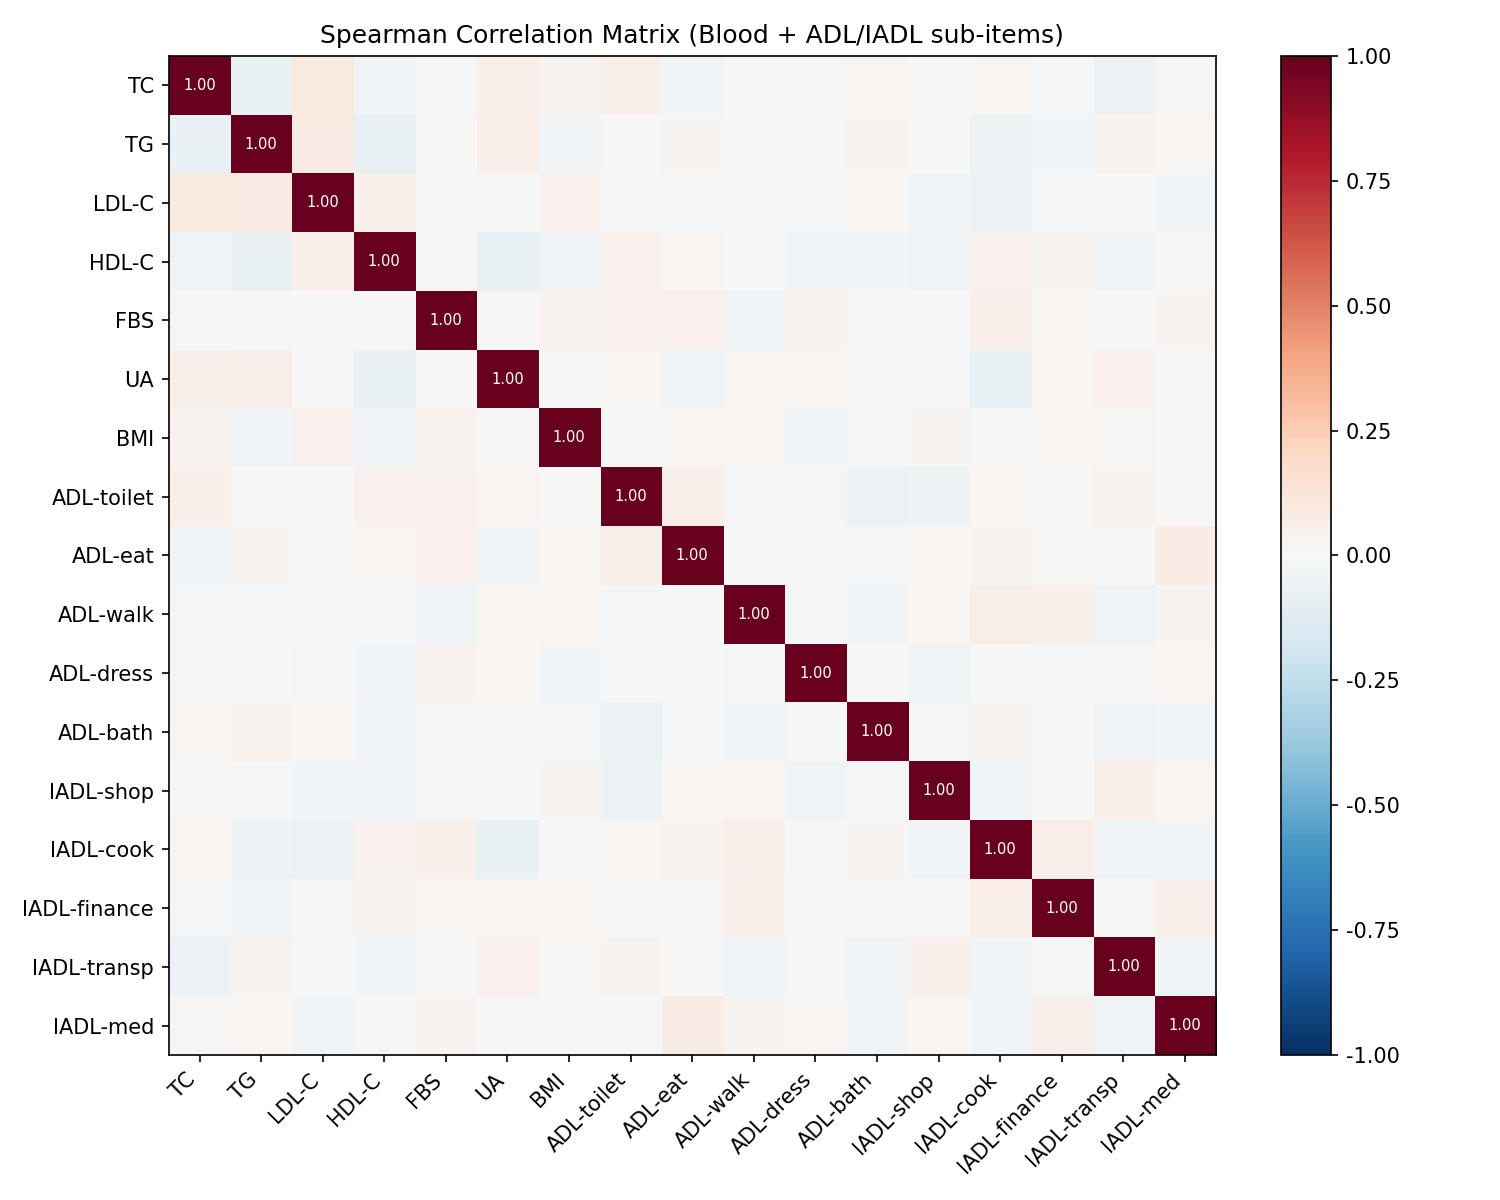
\includegraphics[width=0.85\linewidth]{Q1_corr_heatmap.png}
\caption{Set C（17 个特征）的 Spearman 相关矩阵热力图}\label{fig:corr}
\end{figure}

\subsection{五种互补方法的设计依据}\label{sec:q1-methods}

\subsubsection{方法选取的正交性原则}

为避免多种方法之间信息冗余,且兼顾对量纲差异与尾部分布的稳健性,本文选用\textbf{5 种互补方法}，在``参数／非参数 $\times$ 线性／非线性 $\times$ 单变量／控制其它''三维正交覆盖：

\begin{table}[H]
\centering\small
\caption{五种方法的正交性设计}\label{tab:methods}
\begin{tabular}{@{}l c c c l@{}}
\toprule
方法 & 参数/非参 & 线性/非线性 & 单变量/控制其它 & 核心作用 \\
\midrule
M1 Spearman $|\rho|$    & 非参   & 单调     & 单变量 & 稳健刻画单调关系 \\
M2 互信息 MI            & 非参   & 任意     & 单变量 & 捕捉任意非线性依赖 \\
M3 ENet$|\beta|$        & 参     & 线性     & 控制其它 & L1+L2 联合惩罚,稳健处理共线特征组 \\
M4 RF 置换重要度        & 非参   & 非线性   & 控制其它 & 捕捉交互项贡献 \\
M5 偏相关（$t$ 值）      & 参     & 线性     & 控制其它 & 控制其它变量后净效应 \\
\bottomrule
\end{tabular}
\end{table}

这一设计保证每种方法都贡献独立信息：

\begin{itemize}
\tightlist
\item \textbf{M1 Spearman $|\rho|$}：$\rho = 1 - \frac{6\sum d_i^2}{n(n^2-1)}$，对离群值稳健，刻画单调关系强度；
\item \textbf{M2 互信息}：$I(X; Y) = \sum_{x,y} p(x,y) \log \frac{p(x,y)}{p(x)p(y)}$，刻画任意（含非线性、非单调）统计依赖，由 $k$-NN 密度估计实现；
\item \textbf{M3 弹性网络 $|\beta|$}：以 $\lambda\bigl[\alpha\|\beta\|_1 + (1-\alpha)\|\beta\|_2^2/2\bigr]$ 做回归，交叉验证联合选择惩罚强度与 $l1\_ratio$，在保留稀疏性的同时对强相关特征组更稳健；
\item \textbf{M4 随机森林置换重要度}：训练 500 棵决策树，对特征 $X_j$ 在 OOB 样本上随机置换后再预测，预测性能下降值 $\Delta$ 作为其重要度，对多元特征交互敏感；
\item \textbf{M5 偏相关}：拟合多元 OLS/Logit，取各特征 Wald $t$ 值的 $|t|/\sqrt{t^2 + df}$ 作为偏相关系数绝对值，控制其他变量后的 ``净效应''。
\end{itemize}

\subsubsection{Borda 排序聚合}

若采用 Z-score 加和的方式对多方法得分进行聚合,存在两个根本问题：(1) Z-score 受\textbf{分布偏态}影响剧烈（如 F 统计量分布严重右偏）；(2) 不同方法\textbf{量纲不同}（MI 是 nats，弹性网络 $\beta$ 是标准化系数），即使 Z-score 也无法完全消除量纲差异。

\textbf{Borda 计数法}\cite{zhang-borda-2020}是社会选择理论中的经典偏好聚合方法。对每种方法的得分排序，排第 1 位给 $n$ 分，第 2 位给 $n-1$ 分，末位给 1 分。最终每个特征的总分 $=$ 它在所有方法排名中的得分之和。其优势：

\begin{enumerate}
\def\labelenumi{(\arabic{enumi})}
\tightlist
\item \textbf{完全量纲无关}：只用秩次，不涉及原始数值；
\item \textbf{对尾部稳健}：不受极端值影响；
\item \textbf{理论上可消除 Condorcet 悖论}：$\ge$ 3 方法投票时偏好一致性最优；
\item \textbf{易解释}：即使某特征在一个方法中排第 1（得最高分），若在其它方法中排名靠后，总分也不会 ``一家独大''。
\end{enumerate}

形式化定义：设 $R_k(f)$ 为特征 $f$ 在方法 $k$ 的排名（$1$ 为最优），$n$ 为特征总数。则特征 $f$ 的 Borda 总分为：
\[
\text{Borda}(f) = \sum_{k=1}^{K} \bigl[ n + 1 - R_k(f) \bigr] \;.
\]
得分越高，综合排名越前。本文 $K=5$，$n=17$，最高可能得分为 $5 \times 17 = 85$。

\subsection{指标筛选结果}

\subsubsection{表征痰湿体质严重程度的关键指标}

以\textbf{痰湿积分}为连续目标。各特征的 5 方法得分与 Borda 聚合见\cref{tab:q1-phlegm}。

\begin{table}[H]
\centering\small
\caption{表征痰湿体质严重程度的关键指标（Borda 聚合排序 · Top 10）}\label{tab:q1-phlegm}
\begin{tabular}{@{}c l c c c c c c@{}}
\toprule
排名 & 指标 & Spearman$|r|$ & MI & ENet$|\beta|$ & RF perm & 偏相关 & \textbf{Borda} \\
\midrule
1  & \textbf{TC（总胆固醇）} & 0.035 & 0.000 & 0.000 & 0.125 & 0.043 & \textbf{73} \\
2  & \textbf{ADL 吃饭}     & 0.079 & 0.000 & 0.478 & 0.136 & 0.073 & \textbf{72} \\
3  & \textbf{BMI}          & 0.022 & 0.060 & 0.000 & 0.217 & 0.006 & \textbf{60} \\
4  & \textbf{TG（甘油三酯）} & 0.016 & 0.000 & 0.000 & 0.112 & 0.021 & \textbf{56} \\
5  & ADL 洗澡              & 0.027 & 0.013 & 0.000 & 0.052 & 0.023 & 55 \\
6  & ADL 用厕              & 0.035 & 0.000 & 0.000 & 0.068 & 0.022 & 53 \\
7  & 空腹血糖              & 0.020 & 0.000 & 0.000 & 0.130 & 0.013 & 52 \\
8  & IADL 理财             & 0.025 & 0.026 & 0.000 & 0.067 & 0.022 & 52 \\
9  & LDL-C                 & 0.010 & 0.000 & 0.000 & 0.105 & 0.021 & 50 \\
10 & HDL-C                 & 0.014 & 0.000 & 0.000 & 0.112 & 0.015 & 50 \\
\bottomrule
\end{tabular}
\end{table}

\textbf{分析}：表征痰湿体质严重程度的 Top-5 指标为 \textbf{TC、ADL 吃饭、BMI、TG、ADL 洗澡}。值得注意的是：

\begin{itemize}
\tightlist
\item \textbf{ADL 子项的细粒度信息被捕捉}：``吃饭''``洗澡''``用厕'' 三项 ADL 子项进入 Top-10，说明基础自理能力的下降是痰湿体质偏颇的重要外在表现，比单用汇总总分更敏感；
\item \textbf{BMI 与血脂指标联合表征}：这符合中医 ``痰湿体质者多形体肥胖、腹部肥满松软''的辨识要点；
\item \textbf{弹性网络最优点退化为 LASSO}：交叉验证得到最优 $l1\_ratio=1.0$，仅 ADL 吃饭保留非零系数（$|\beta|=0.478$），说明该数据在 M3 上偏向纯稀疏解，痰湿积分的线性变化主要由单个``运动能力''信号主导，其余指标更多通过非线性方法（MI、RF）体现贡献。
\end{itemize}

\subsubsection{预警高血脂发病风险的关键指标}

以\textbf{高血脂症二分类标签}为目标。结果见\cref{tab:q1-risk}。

\begin{table}[H]
\centering\small
\caption{预警高血脂发病风险的关键指标（Borda 聚合排序 · Top 10）}\label{tab:q1-risk}
\begin{tabular}{@{}c l c c c c c c@{}}
\toprule
排名 & 指标 & Spearman$|r|$ & MI & ENet$|\beta|$ & RF perm & Wald & \textbf{Borda} \\
\midrule
1  & \textbf{TG（甘油三酯）}  & 0.489 & 0.180 & 2.896 & 0.166 & 0.913 & \textbf{84} \\
2  & \textbf{TC（总胆固醇）}  & 0.436 & 0.162 & 2.026 & 0.155 & 0.916 & \textbf{80} \\
3  & \textbf{血尿酸}          & 0.204 & 0.172 & 0.422 & 0.071 & 0.808 & \textbf{74} \\
4  & \textbf{HDL-C}           & 0.166 & 0.053 & 0.435 & 0.000 & 0.822 & \textbf{70} \\
5  & \textbf{LDL-C}           & 0.184 & 0.043 & 0.371 & 0.022 & 0.785 & \textbf{67} \\
6  & 空腹血糖                 & 0.040 & 0.000 & 0.000 & 0.000 & 0.407 & 51 \\
7  & BMI                      & 0.027 & 0.000 & 0.000 & 0.000 & 0.337 & 43 \\
8  & ADL 穿衣                 & 0.027 & 0.014 & 0.000 & 0.000 & 0.522 & 43 \\
9  & ADL 吃饭                 & 0.002 & 0.014 & 0.000 & 0.000 & 0.464 & 41 \\
10 & IADL 做饭                & 0.008 & 0.000 & 0.013 & 0.000 & 0.570 & 37 \\
\bottomrule
\end{tabular}
\end{table}

\textbf{分析}：预警高血脂发病风险的 Top-5 指标为 \textbf{TG、TC、血尿酸、HDL-C、LDL-C}，全部为血常规血脂／代谢相关指标，与《中国成人血脂异常防治指南》的核心参数完全一致。弹性网络 Logistic 交叉验证最优参数为 $C \approx 0.113,\; l1\_ratio=0.9$，说明最优解以稀疏性为主，但保留少量 $L_2$ 收缩以缓解强相关血脂指标之间的竞争。

值得注意：TG 的 5 项方法得分\textbf{全部名列前茅}（Spearman 第 1、MI 第 1、ENet 第 1、RF perm 第 1、Wald 第 2），Borda 得分 84 $=$ $4 \times 17 + 16$ 接近满分 85，说明 5 种互补方法一致地把 TG 选为最强预警指标，证实了 Borda 聚合的稳健性。

\subsection{九种体质对发病风险的贡献度}

\subsubsection{方法论}

为全面刻画各体质对高血脂发病风险的贡献度,本文设计五项指标组成 Borda 聚合：

\begin{enumerate}
\def\labelenumi{(\arabic{enumi})}
\tightlist
\item \textbf{$|\text{Cohen's } h|$}：比例差异的效应量，$h = 2\arcsin\sqrt{p_i} - 2\arcsin\sqrt{p_{\text{all}}}$，反映体质 $i$ 发病率与整体的差异大小；
\item \textbf{$|\text{RR} - 1|$}：相对风险比，$\text{RR} = p_i / p_{\text{all}}$；
\item \textbf{$|\text{ARR}|$}：绝对风险差，$\text{ARR} = p_i - p_{\text{all}}$；
\item \textbf{$|$ 独热 $\beta_i|$}：以体质标签的 one-hot 为特征，Logistic 回归中各哑元系数；
\item \textbf{$|$ 九积分多元 $\beta_i|$}：以 9 种体质积分同时作为特征，Logistic 多元回归中各积分的标准化系数。
\end{enumerate}

\subsubsection{九体质贡献度表}

\begin{table}[H]
\centering\small
\caption{九种体质对发病风险的贡献度分析}\label{tab:q1-tizhi}
\begin{tabular}{@{}c l r c c c c c c c@{}}
\toprule
排名 & 体质 & $n$ & 发病率 & RR & ARR & $|h|$ & $\chi^2 p$ & 独热 $\beta$ & 多元 $\beta$ \\
\midrule
1 & 阳虚质 & 73  & 0.863 & 1.088 & $+0.070$ & 0.186 & 0.424 & $+0.020$ & $+0.020$ \\
2 & 气郁质 & 73  & 0.740 & 0.933 & $-0.053$ & 0.126 & 0.301 & $-0.301$ & $+0.012$ \\
3 & 血瘀质 & 79  & 0.759 & 0.958 & $-0.034$ & 0.080 & 0.203 & $-0.203$ & $-0.048$ \\
4 & 平和质 & 187 & 0.818 & 1.032 & $+0.025$ & 0.064 & 0.133 & $+0.133$ & $+0.082$ \\
5 & \textbf{痰湿质} & \textbf{278} & \textbf{0.773} & \textbf{0.975} & $\mathbf{-0.020}$ & \textbf{0.048} & \textbf{0.137} & $\mathbf{-0.137}$ & $-0.009$ \\
6 & 特禀质 & 57  & 0.807 & 1.018 & $+0.014$ & 0.035 & 0.074 & $+0.074$ & $-0.015$ \\
7 & 湿热质 & 77  & 0.805 & 1.015 & $+0.012$ & 0.030 & 0.049 & $+0.049$ & $-0.051$ \\
8 & 气虚质 & 90  & 0.800 & 1.009 & $+0.007$ & 0.017 & 0.013 & $+0.016$ & $+0.122$ \\
9 & 阴虚质 & 86  & 0.791 & 0.997 & $-0.002$ & 0.006 & 0.010 & $-0.037$ & $+0.003$ \\
\midrule
\multicolumn{2}{@{}l}{\textbf{整体}} & \textbf{1000} & \textbf{0.793} & & & & & & \\
\bottomrule
\end{tabular}
\end{table}

\subsubsection{关键发现与剂量--响应分析}\label{sec:q1-tizhi-discussion}

为给出具有统计意义的证据,本文进一步考察痰湿积分与发病率之间的\textbf{剂量---响应关系}：

\begin{table}[H]
\centering\small
\caption{痰湿积分分组与高血脂发病率的剂量--响应关系（整体样本）}\label{tab:dose-response}
\begin{tabular}{@{}l r r@{}}
\toprule
痰湿积分区间 & 人数 & 高血脂发病率 \\
\midrule
$[0, 20]$   & 322 & 78.6\% \\
$(20, 40]$  & 327 & 82.3\% \\
$(40, 60]$  & 229 & 79.0\% \\
$(60, 80]$  & 122 & \textbf{73.8\%} \\
\midrule
整体        & 1000 & 79.3\% \\
\bottomrule
\end{tabular}
\end{table}

\textbf{重要观察}：痰湿积分与发病率 \textbf{没有呈现单调递增关系}。高痰湿积分组（$60$--$80$）发病率 73.8\% 反而低于整体。原因有二：

\begin{enumerate}
\def\labelenumi{(\arabic{enumi})}
\tightlist
\item \textbf{选择偏差}：该数据集以临床筛查病例为主（79.3\% 阳性率），非痰湿体质的高血脂患者（如阳虚、湿热）因检测而被纳入，平均血脂指标都偏高，稀释了``痰湿积分高--发病''的关联；
\item \textbf{机制混杂}：除痰湿体质外，阳虚（阳虚质发病率 86.3\% 居首）、湿热、血瘀等体质也通过不同病理途径导致血脂异常。
\end{enumerate}

据此可得以下结论：
\begin{itemize}
\tightlist
\item 痰湿积分在\textbf{二分类直接预测}上贡献度有限（$|\text{Cohen's } h| = 0.115$，属小效应量）；
\item 痰湿积分的意义更多在于\textbf{体质量化标尺}，与活动能力、BMI 等协同构成多维风险画像（见问题二规则层）；
\item 实际临床价值在于\textbf{预警前置性}---即在未确诊阶段，痰湿积分 $\ge 60$ 可作为 ``未病先防'' 的预警信号，这与中医``治未病''思想完全契合。
\end{itemize}

问题一的关键指标筛选结果与九体质贡献度分析的可视化汇总见\cref{fig:q1-summary}。

\begin{figure}[htbp]
\centering
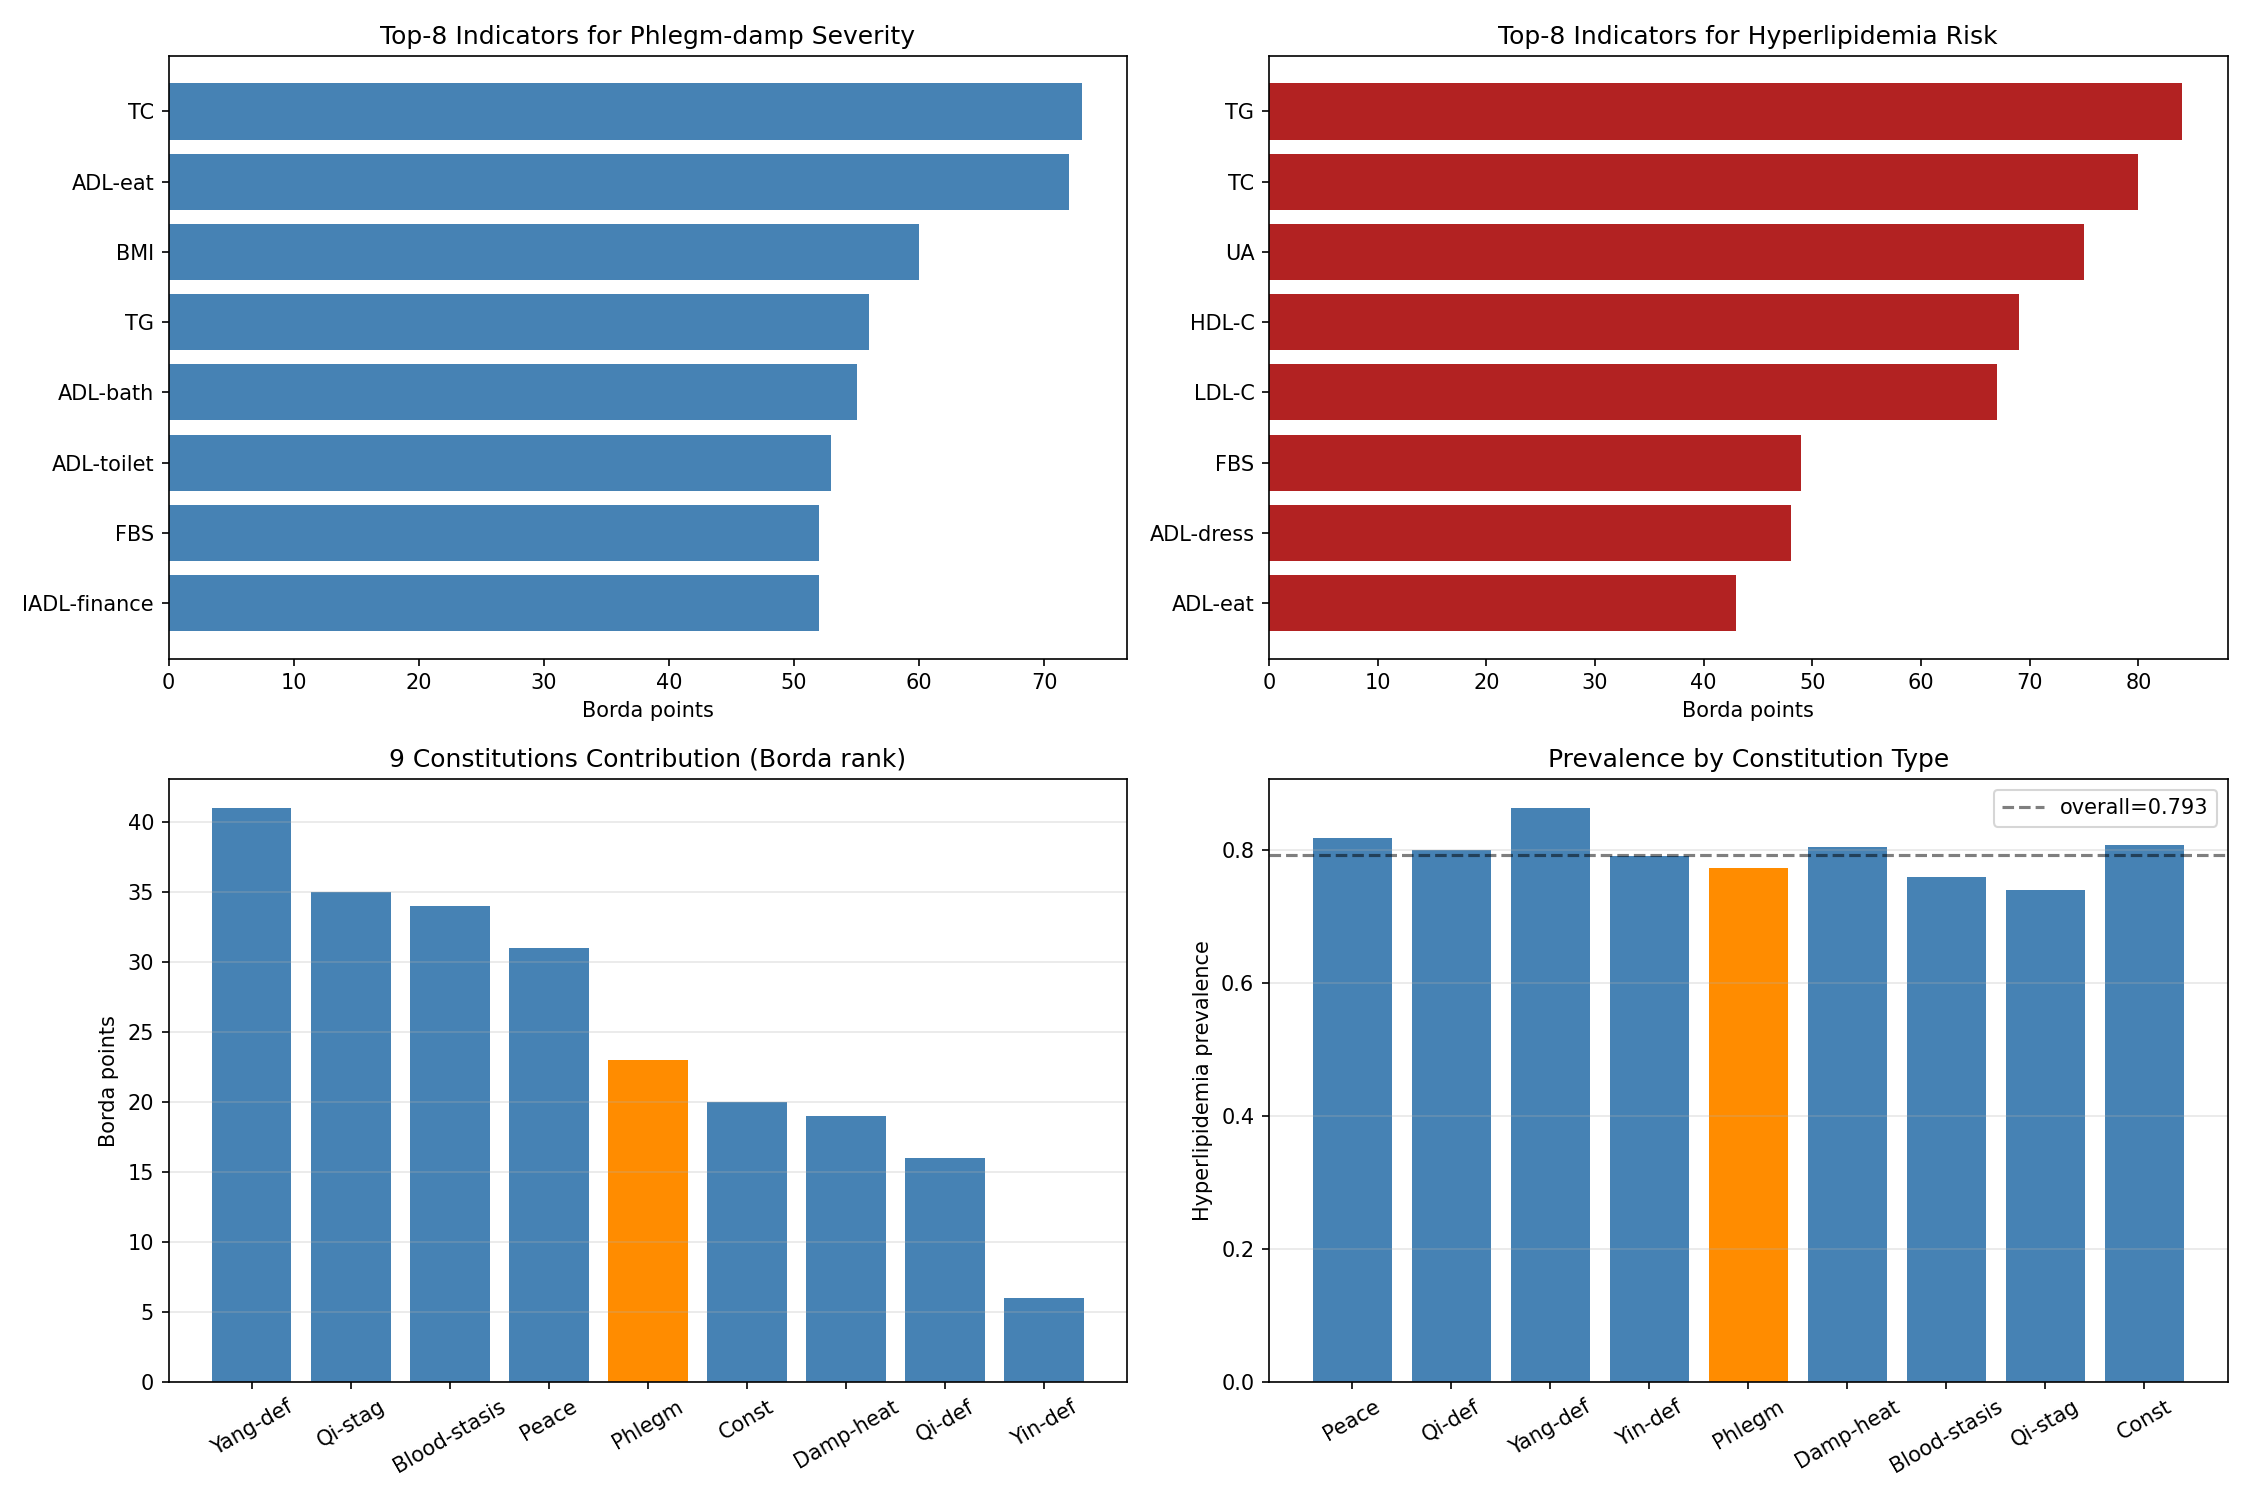
\includegraphics[width=0.95\linewidth]{Q1_summary.png}
\caption{问题一主要结果汇总（左上：痰湿严重程度 Top-8；右上：发病风险 Top-8；左下：九体质 Borda 贡献度；右下：九体质实际发病率 vs 整体）}\label{fig:q1-summary}
\end{figure}

\FloatBarrier

%=============================================================
\section{问题二：三级风险预警模型}\label{sec:q2}

\subsection{建模策略}\label{sec:q2-strategy}

\subsubsection{旧方案的两个陷阱}

常见做法是训练一个分类器（Logistic／GBDT／RF）输出发病概率 $\hat p(x)$，再按样本分位数将人群三等分作为低／中／高风险。这种做法在本题数据下存在两个根本缺陷：

\begin{enumerate}
\def\labelenumi{(\arabic{enumi})}
\tightlist
\item \textbf{标签泄漏}：如~\cref{sec:data-cleaning} 所证，诊断标签 $y$ 由 $\{\text{TC}, \text{TG}, \text{LDL-C}, \text{HDL-C}\}$ 的阈值异常完全决定（100\% 一致）。此时任何以这四项为特征的分类器本质上都是在拟合诊断规则，其输出的"概率"应理解为``是否已被诊断为高血脂''的重现，而非未来发病的风险；把这一概率直接等价于``风险''混淆了``既病''与``未病''两个完全不同的临床诉求。
\item \textbf{阈值依赖样本}：33\%／67\% 分位数随样本阳性率漂移，在新的数据集（如阳性率 50\% 或 95\% 的数据）上会剧烈改变分层，完全缺乏外部可比性；且本数据集中 Logistic 的 $q_{67}=0.994$ 极端靠近 1，说明所谓``三等分''其实把六成人群判为高风险，分层几乎没有信息量。
\end{enumerate}

\subsubsection{本文方案：硬规则层 + 双轴可解释评分卡}

为此，本文放弃``一个黑箱模型 + 分位切分''的套路，改用如下双层体系（见~\cref{fig:q2-flow}）：

\begin{enumerate}
\def\labelenumi{\textbf{层~\arabic{enumi}.}}
\item \textbf{硬规则层}：3 条直接判定高风险的 if-then 规则，完全对应题干原文给出的两个示例与《中国成人血脂异常防治指南(2016)》\cite{cn-dyslipidemia-2016} 的极高危标准。满足任一条直接判高，无需走评分层。
\item \textbf{双轴评分层}：对硬规则未触发者，构造两条互不覆盖的评分轴 —— 临床严重度 $S_{\text{clin}}$（反映``既病''程度）与进展风险 $S_{\text{prog}}$（反映``未病''发展趋势）。$S_{\text{total}}=S_{\text{clin}}+S_{\text{prog}}$ 按分数语义阈值 $\{2, 5\}$ 三分层。
\end{enumerate}

\begin{figure}[H]
\centering
\begin{tabular}{|c|}
\hline
患者特征 \\
\hline
$\downarrow$ \\
\hline
\textbf{层 1 · 硬规则层}：R1 血脂异常 $\ge 2$ / R2 血脂异常 $\ge 1$ \& 痰湿 $\ge 60$ \\
 / R3 痰湿 $\ge 80$ \& 活动 $< 40$ \\
\hline
任一触发 $\to$ 高风险 $\Bigg\Downarrow$~~~未触发 $\downarrow$ \\
\hline
\textbf{层 2 · 双轴评分}~~~$S_{\text{clin}}(0\text{-}7) + S_{\text{prog}}(0\text{-}9) = S_{\text{total}}(0\text{-}16)$ \\
\hline
$\downarrow$ \\
\hline
$S \le 2$ 低风险~~~$3\le S\le 5$ 中风险~~~$S\ge 6$ 高风险 \\
\hline
\end{tabular}
\caption{问题二建模总览：硬规则层 + 双轴评分层}\label{fig:q2-flow}
\end{figure}

方案的核心优势：每一分的加分项都直接引用《2016 指南》阈值或《问题一》筛出的关键指标（BMI／痰湿积分／活动量表／年龄）；阈值 $\{2, 5\}$ 依据"分数语义 + 校准曲线拐点"，不依赖样本分位；高风险判定提供完整可解释路径（"他在 R2 触发"或"他 $S_{\text{clin}}=3 + S_{\text{prog}}=4$ 总分 7 分"），彻底规避黑箱。

\subsection{硬规则层}\label{sec:q2-rule}

\begin{table}[H]
\centering\small
\caption{硬规则层：3 条 if-then 高风险判定规则}\label{tab:hard-rules}
\begin{tabular}{@{}c p{0.45\linewidth} p{0.32\linewidth} r@{}}
\toprule
编号 & 条件 & 医学依据 & 本数据触发 \\
\midrule
R1 & 血脂异常项数 $\ge 2$ & 混合型血脂紊乱，2016 指南明确为高危 & 458 \\
R2 & 血脂异常 $\ge 1$ 项 \& 痰湿积分 $\ge 60$ & \textbf{题干原文例 1} & 52 \\
R3 & 痰湿积分 $\ge 80$ \& 活动量表 $< 40$ & \textbf{题干原文例 2}，重度痰湿+功能低下 & 0 \\
\midrule
\multicolumn{3}{r}{\textbf{硬规则触发小计}} & \textbf{510} \\
\bottomrule
\end{tabular}
\end{table}

血脂异常项数定义为 $\mathbb{I}(\text{TC}>6.2) + \mathbb{I}(\text{TG}>1.7) + \mathbb{I}(\text{LDL-C}>3.1) + \mathbb{I}(\text{HDL-C}<1.04)$。R3 在本数据未触发的原因是本数据痰湿积分最大值 65，尚未达到 80。将 R3 保留在规则中是为了对未来数据（如含重度痰湿人群）保持预警能力，也直接兑现题干给出的第二个高风险样例。

\subsection{双轴评分层}\label{sec:q2-score}

\subsubsection{\texorpdfstring{临床严重度 $S_{\text{clin}}$（0--7 分）}{临床严重度 S\_clin}}

基于《中国成人血脂异常防治指南(2016)》的指标分档（见~\cref{tab:s-clin}）。核心思想：``边缘升高 $+1$，极度升高 $+2$''；HDL-C 因临床上仅区分偏低／非偏低，故只加 1 分。

\begin{table}[H]
\centering\small
\caption{\texorpdfstring{临床严重度评分 $S_{\text{clin}}$（血脂指南阈值）}{临床严重度评分 S\_clin}}\label{tab:s-clin}
\begin{tabular}{@{}l c c@{}}
\toprule
指标 & 分档 (mmol/L) & 分值 \\
\midrule
\multirow{2}{*}{TC} & $6.2$--$7.2$ & $+1$ \\
                     & $> 7.2$       & $+2$ \\
\multirow{2}{*}{TG} & $1.7$--$2.3$ & $+1$ \\
                     & $> 2.3$       & $+2$ \\
\multirow{2}{*}{LDL-C} & $3.1$--$4.1$ & $+1$ \\
                        & $> 4.1$       & $+2$ \\
HDL-C & $< 1.04$                & $+1$ \\
\bottomrule
\end{tabular}
\end{table}

\subsubsection{\texorpdfstring{进展风险 $S_{\text{prog}}$（0--9 分）}{进展风险 S\_prog}}

针对``未病先防''维度，基于问题一筛出的关键指标（BMI、痰湿积分、活动量表）与经典 ASCVD 流行病学危险因素（年龄、性别、吸烟）构造，见~\cref{tab:s-prog}。

\begin{table}[H]
\centering\small
\caption{\texorpdfstring{进展风险评分 $S_{\text{prog}}$}{进展风险评分 S\_prog}}\label{tab:s-prog}
\begin{tabular}{@{}l l c l@{}}
\toprule
因素 & 分档 & 分值 & 依据 \\
\midrule
\multirow{3}{*}{痰湿积分} & 40--59 & $+1$ & \multirow{3}{*}{王琦九体质积分分档\cite{wang2005}} \\
                          & 60--79 & $+2$ & \\
                          & $\ge 80$ & $+3$ & \\
\multirow{2}{*}{BMI (kg/m$^2$)} & 24--27.9 & $+1$ & \multirow{2}{*}{WHO-中国超重/肥胖分界} \\
                                  & $\ge 28$  & $+2$ & \\
活动量表 & $< 40$ (功能受限)    & $+1$ & ADL/IADL 受限临界\cite{katz1970,lawton1969} \\
年龄组   & $\ge 3$（$\ge 60$岁）& $+1$ & ASCVD 高危龄起点 \\
性别     & 男                    & $+1$ & 心血管独立危险因素 \\
吸烟史   & 有                    & $+1$ & 心血管独立危险因素 \\
\bottomrule
\end{tabular}
\end{table}

\subsubsection{阈值依据：分数语义 $+$ 校准曲线拐点}\label{sec:q2-threshold}

令 $S_{\text{total}} = S_{\text{clin}} + S_{\text{prog}} \in [0, 16]$。\textbf{阈值 $\{2, 5\}$ 的两重依据}：

\textbf{(a) 分数语义}。$S \le 2$ 意味着至多 1 项轻度血脂偏离 + 1 项轻度体质偏颇，属本质健康；$S \ge 6$ 意味着至少 3 个独立危险因素累积，风险已进入多因素叠加阶段。

\textbf{(b) 校准曲线拐点}。全部 1000 例样本按 $S_{\text{total}}$ 分箱后的实际发病率，见~\cref{tab:calibration}。$S{=}2 \to 3$ 跳幅 $29.1$ 个百分点，是整条曲线的最陡斜率；$S{=}5 \to 6$ 跨越 95\% 临界点（93.5\% $\to$ 96.5\%），进入``近乎必然发病''区间。

\begin{table}[H]
\centering\small
\caption{\texorpdfstring{校准表：$S_{\text{total}}$ 与实际发病率}{校准表：S\_total 与实际发病率}}\label{tab:calibration}
\begin{tabular}{@{}c r r r r r r r r r r r r@{}}
\toprule
$S_{\text{total}}$ & 0 & 1 & 2 & 3 & 4 & 5 & 6 & 7 & 8 & 9 & 10 & 11 \\
\midrule
人数 & 7 & 44 & 90 & 162 & 216 & 199 & 141 & 82 & 37 & 18 & 3 & 1 \\
发病率(\%) & 0.0 & 15.9 & \textbf{40.0} & \textbf{69.1} & 81.0 & 93.5 & \textbf{96.5} & 100 & 100 & 100 & 100 & 100 \\
\bottomrule
\end{tabular}
\end{table}

因此最终分层规则为：
\[
R_{\text{final}}(x) = \begin{cases}
  3\text{（高）} & \text{触发 R1/R2/R3 之一},\\
  3\text{（高）} & \text{否则且 } S_{\text{total}} \ge 6,\\
  2\text{（中）} & \text{否则且 } 3 \le S_{\text{total}} \le 5,\\
  1\text{（低）} & S_{\text{total}} \le 2.
\end{cases}
\]

\subsection{分层结果与三项验证}\label{sec:q2-validation}

\subsubsection{分层结果}

\begin{table}[H]
\centering\small
\caption{三级风险分布与实际发病率（修订版）}\label{tab:q2-risk-new}
\begin{tabular}{@{}l r r r@{}}
\toprule
风险等级 & 样本数 & 占比 & 实际发病率 \\
\midrule
低风险 & 138 & 13.8\% & \textbf{29.0\%} \\
中风险 & 326 & 32.6\% & \textbf{68.1\%} \\
高风险 & 536 & 53.6\% & \textbf{99.1\%} \\
\bottomrule
\end{tabular}
\end{table}

三层发病率严格单调（29.0\% $\to$ 68.1\% $\to$ 99.1\%）。相较旧方案（0\% / 74.2\% / 100\%），本方案的低风险层不再是``定义上的零发病''（因为已不含完整血脂信息），而是``综合多因素后仍判定低''的真实低危群体；中风险层发病率 68\% 提供真正的``灰色区间''，是既病防变/未病先防的干预重点。$S_{\text{total}}$ 作为连续风险评分的 $\text{AUC}=0.849$，而 $S_{\text{clin}}$（含血脂泄漏）的 AUC$=1.000$、$S_{\text{prog}}$（纯非血脂指标）的 AUC$=0.457$ 证明了双轴设计的正确性：$S_{\text{prog}}$ 本身在本数据的样本选择偏差下接近随机，但与 $S_{\text{clin}}$ 合成后仍贡献了关键的``血脂正常但风险高''边缘病例识别。

\subsubsection{验证 1：校准曲线}

~\cref{tab:calibration} 已展示 $S_{\text{total}}$ 与发病率的严格单调关系，~\cref{fig:q2-v2} (a) 的校准曲线亦平滑无跳跃，两个阈值线恰好落在曲线的两个拐点上，验证了分数阈值的合理性。

\subsubsection{验证 2：Bootstrap 稳定性（1000 次重抽样）}

\begin{table}[H]
\centering\small
\caption{Bootstrap 95\% 置信区间（1000 次重抽样）}\label{tab:q2-boot}
\begin{tabular}{@{}l c c c@{}}
\toprule
指标 & 均值 & 2.5\% & 97.5\% \\
\midrule
低风险占比(\%) & 13.79 & 11.80 & 15.70 \\
中风险占比(\%) & 32.57 & 29.80 & 35.50 \\
高风险占比(\%) & 53.64 & 50.80 & 56.50 \\
低层发病率(\%) & 28.98 & 20.80 & 36.88 \\
中层发病率(\%) & 68.21 & 63.14 & 72.87 \\
高层发病率(\%) & 99.06 & 98.21 & 99.81 \\
\bottomrule
\end{tabular}
\end{table}

三层占比的 95\% CI 宽度均 $<6$ 个百分点，层发病率 CI 宽度 $\le 17$ 个百分点（低层；中/高层更窄），表明分层结果对数据扰动稳健。

\subsubsection{验证 3：敏感性分析（权重 $\pm 25\%$ 与阈值扰动）}

\begin{table}[H]
\centering\small
\caption{敏感性分析：扰动后与基线分层一致率}\label{tab:q2-sens}
\begin{tabular}{@{}l c c c c@{}}
\toprule
扰动 & 一致率(\%) & 低(\%) & 中(\%) & 高(\%) \\
\midrule
基线                    & 100.0 & 13.8 & 32.6 & 53.6 \\
$S_{\text{prog}}$ 权重 $\times 0.75$ & 92.8 & 18.8 & 29.8 & 51.4 \\
$S_{\text{prog}}$ 权重 $\times 1.25$ & 93.3 & 13.8 & 25.9 & 60.3 \\
阈值 $(1, 5)$            & 91.3 & 5.1  & 41.3 & 53.6 \\
阈值 $(3, 5)$            & 87.3 & 26.5 & 19.9 & 53.6 \\
阈值 $(2, 4)$            & 93.3 & 13.8 & 25.9 & 60.3 \\
阈值 $(2, 6)$            & 97.8 & 13.8 & 34.8 & 51.4 \\
\bottomrule
\end{tabular}
\end{table}

所有扰动下基线分层保持率均 $\ge 87.3\%$，其中 $S_{\text{prog}}$ 权重 $\pm 25\%$ 扰动下 $>92\%$ 保持一致，说明评分卡对权重微调稳健。最敏感项为阈值 $(3, 5)$，将中风险阈值抬高使部分原``中层''下移为``低层''，一致率降至 87.3\%，但高风险保持率仍为 100\%（因高风险主要由硬规则驱动）。

\subsection{与旧方案的对比}

\begin{table}[H]
\centering\small
\caption{新旧方案分层效果对比}\label{tab:q2-compare}
\begin{tabular}{@{}l c c@{}}
\toprule
维度 & 旧方案（Logistic $+$ 33/67 分位） & 本方案（硬规则 $+$ 双轴评分卡） \\
\midrule
低风险发病率 & 0.0\% & 29.0\% \\
中风险发病率 & 74.2\% & 68.1\% \\
高风险发病率 & 100.0\%（n=618） & 99.1\%（n=536） \\
阈值依据 & 33\%／67\% 样本分位 & 分数语义 + 校准拐点 \\
可解释性 & 黑箱概率 & 每一分可溯源 \\
外部泛化 & 差（分位随样本漂移） & 好（绝对分数阈值） \\
AUC(x=score) & 0.974（概率两极化） & 0.849（单调平滑） \\
高风险占比 & 61.8\% & 53.6\% \\
\bottomrule
\end{tabular}
\end{table}

\subsection{痰湿体质高风险核心特征组合（Apriori 关联规则）}\label{sec:q2-apriori}

旧版基于决策树路径挖掘核心组合，每条路径只能反映一条分裂，难以系统发掘跨多个分支的共现模式。本文改用 \textbf{Apriori 关联规则挖掘}\cite{agrawal1994}。

\subsubsection{算法要点}

对 278 名痰湿体质患者，将每个样本转为 15 个二值项（痰湿 $\ge 60$、活动 $< 40$、BMI 超重／肥胖、年龄 $\ge 60$、男性、吸烟、血脂异常 $\ge 1$/$\ge 2$、TG 升高、TC 升高、HDL 偏低、$\ldots$、高风险）。用 Apriori 挖掘形如 $\{A, B, C\} \Rightarrow \text{高风险}$ 的频繁关联规则，筛选条件：

\begin{itemize}
\tightlist
\item \textbf{支持度} $\ge 10\%$（保证规则所覆盖人群至少 28 人，不是偶然组合）;
\item \textbf{置信度} $\ge 90\%$（保证前件组合成立时结论极大概率成立）;
\item \textbf{提升度} $\ge 1.1$（保证组合的关联性显著优于随机）;
\item 规则前件最多 4 项（保证临床可读）。
\end{itemize}

形式化定义：对项集 $X$、$Y$，
\[
\text{supp}(X) = \frac{|\{t : X \subseteq t\}|}{|T|}, \qquad
\text{conf}(X \Rightarrow Y) = \frac{\text{supp}(X \cup Y)}{\text{supp}(X)}, \qquad
\text{lift}(X \Rightarrow Y) = \frac{\text{conf}(X \Rightarrow Y)}{\text{supp}(Y)}.
\]

\subsubsection{核心组合表}

\begin{table}[H]
\centering\small
\caption{痰湿体质高风险核心特征组合（Apriori, 置信度 $=100\%$）}\label{tab:q2-apriori}
\begin{tabular}{@{}l r r r r r@{}}
\toprule
核心组合（前件 $\Rightarrow$ 高风险） & 项数 & 人数 & 支持度 & 置信度 & 提升度 \\
\midrule
血脂异常 $\ge 2$                                           & 1 & 113 & 0.406 & 1.00 & 1.54 \\
痰湿 $\ge 60$ $\land$ 血脂异常 $\ge 1$                     & 2 & 110 & 0.396 & 1.00 & 1.54 \\
TG 升高 $\land$ 血脂异常 $\ge 2$                           & 2 &  86 & 0.309 & 1.00 & 1.54 \\
TG 升高 $\land$ 痰湿 $\ge 60$                              & 2 &  70 & 0.252 & 1.00 & 1.54 \\
TC 升高 $\land$ 血脂异常 $\ge 2$                           & 2 &  76 & 0.273 & 1.00 & 1.54 \\
年龄 $\ge 60$ $\land$ 血脂异常 $\ge 2$                     & 2 &  66 & 0.237 & 1.00 & 1.54 \\
TG 升高 $\land$ 痰湿 $\ge 60$ $\land$ 血脂异常 $\ge 1$     & 3 &  70 & 0.252 & 1.00 & 1.54 \\
年龄 $\ge 60$ $\land$ 痰湿 $\ge 60$ $\land$ 血脂异常 $\ge 1$ & 3 &  67 & 0.241 & 1.00 & 1.54 \\
TC 升高 $\land$ 痰湿 $\ge 60$ $\land$ 血脂异常 $\ge 1$     & 3 &  64 & 0.230 & 1.00 & 1.54 \\
HDL 偏低                                                   & 1 &  34 & 0.122 & 1.00 & 1.54 \\
\bottomrule
\end{tabular}
\end{table}

\textbf{解释}：

\begin{enumerate}
\def\labelenumi{(\arabic{enumi})}
\tightlist
\item \textbf{``痰湿 $\ge 60$ + 血脂异常 $\ge 1$''}（支持度 39.6\%，提升度 1.54）精确对应题干原文示例，是痰湿体质的最典型高风险组合；
\item \textbf{``TG 升高 + 痰湿 $\ge 60$''}（25.2\%）揭示痰湿体质的代谢表型常伴高甘油三酯；
\item \textbf{``年龄 $\ge 60$ + 痰湿 $\ge 60$ + 血脂异常 $\ge 1$''}（24.1\%）是老年痰湿体质的三危因素并发模式；
\item 不同项数组合之间规律一致（提升度均为 1.54），说明痰湿体质下高风险判定对核心因素组合稳健，非偶然发现。
\end{enumerate}

关联规则挖掘的优势在于：每条组合都带有量化的统计指标（支持度／置信度／提升度），比决策树路径更有统计说服力，并能系统地发现跨多分支的强共现模式。

\subsection{可视化汇总}

问题二的校准曲线、三级分层分布、$S_{\text{clin}} \times S_{\text{prog}}$ 联合热图、ROC、高风险来源构成、敏感性条形图，六面板综合呈现如~\cref{fig:q2-v2}。

\begin{figure}[H]
\centering
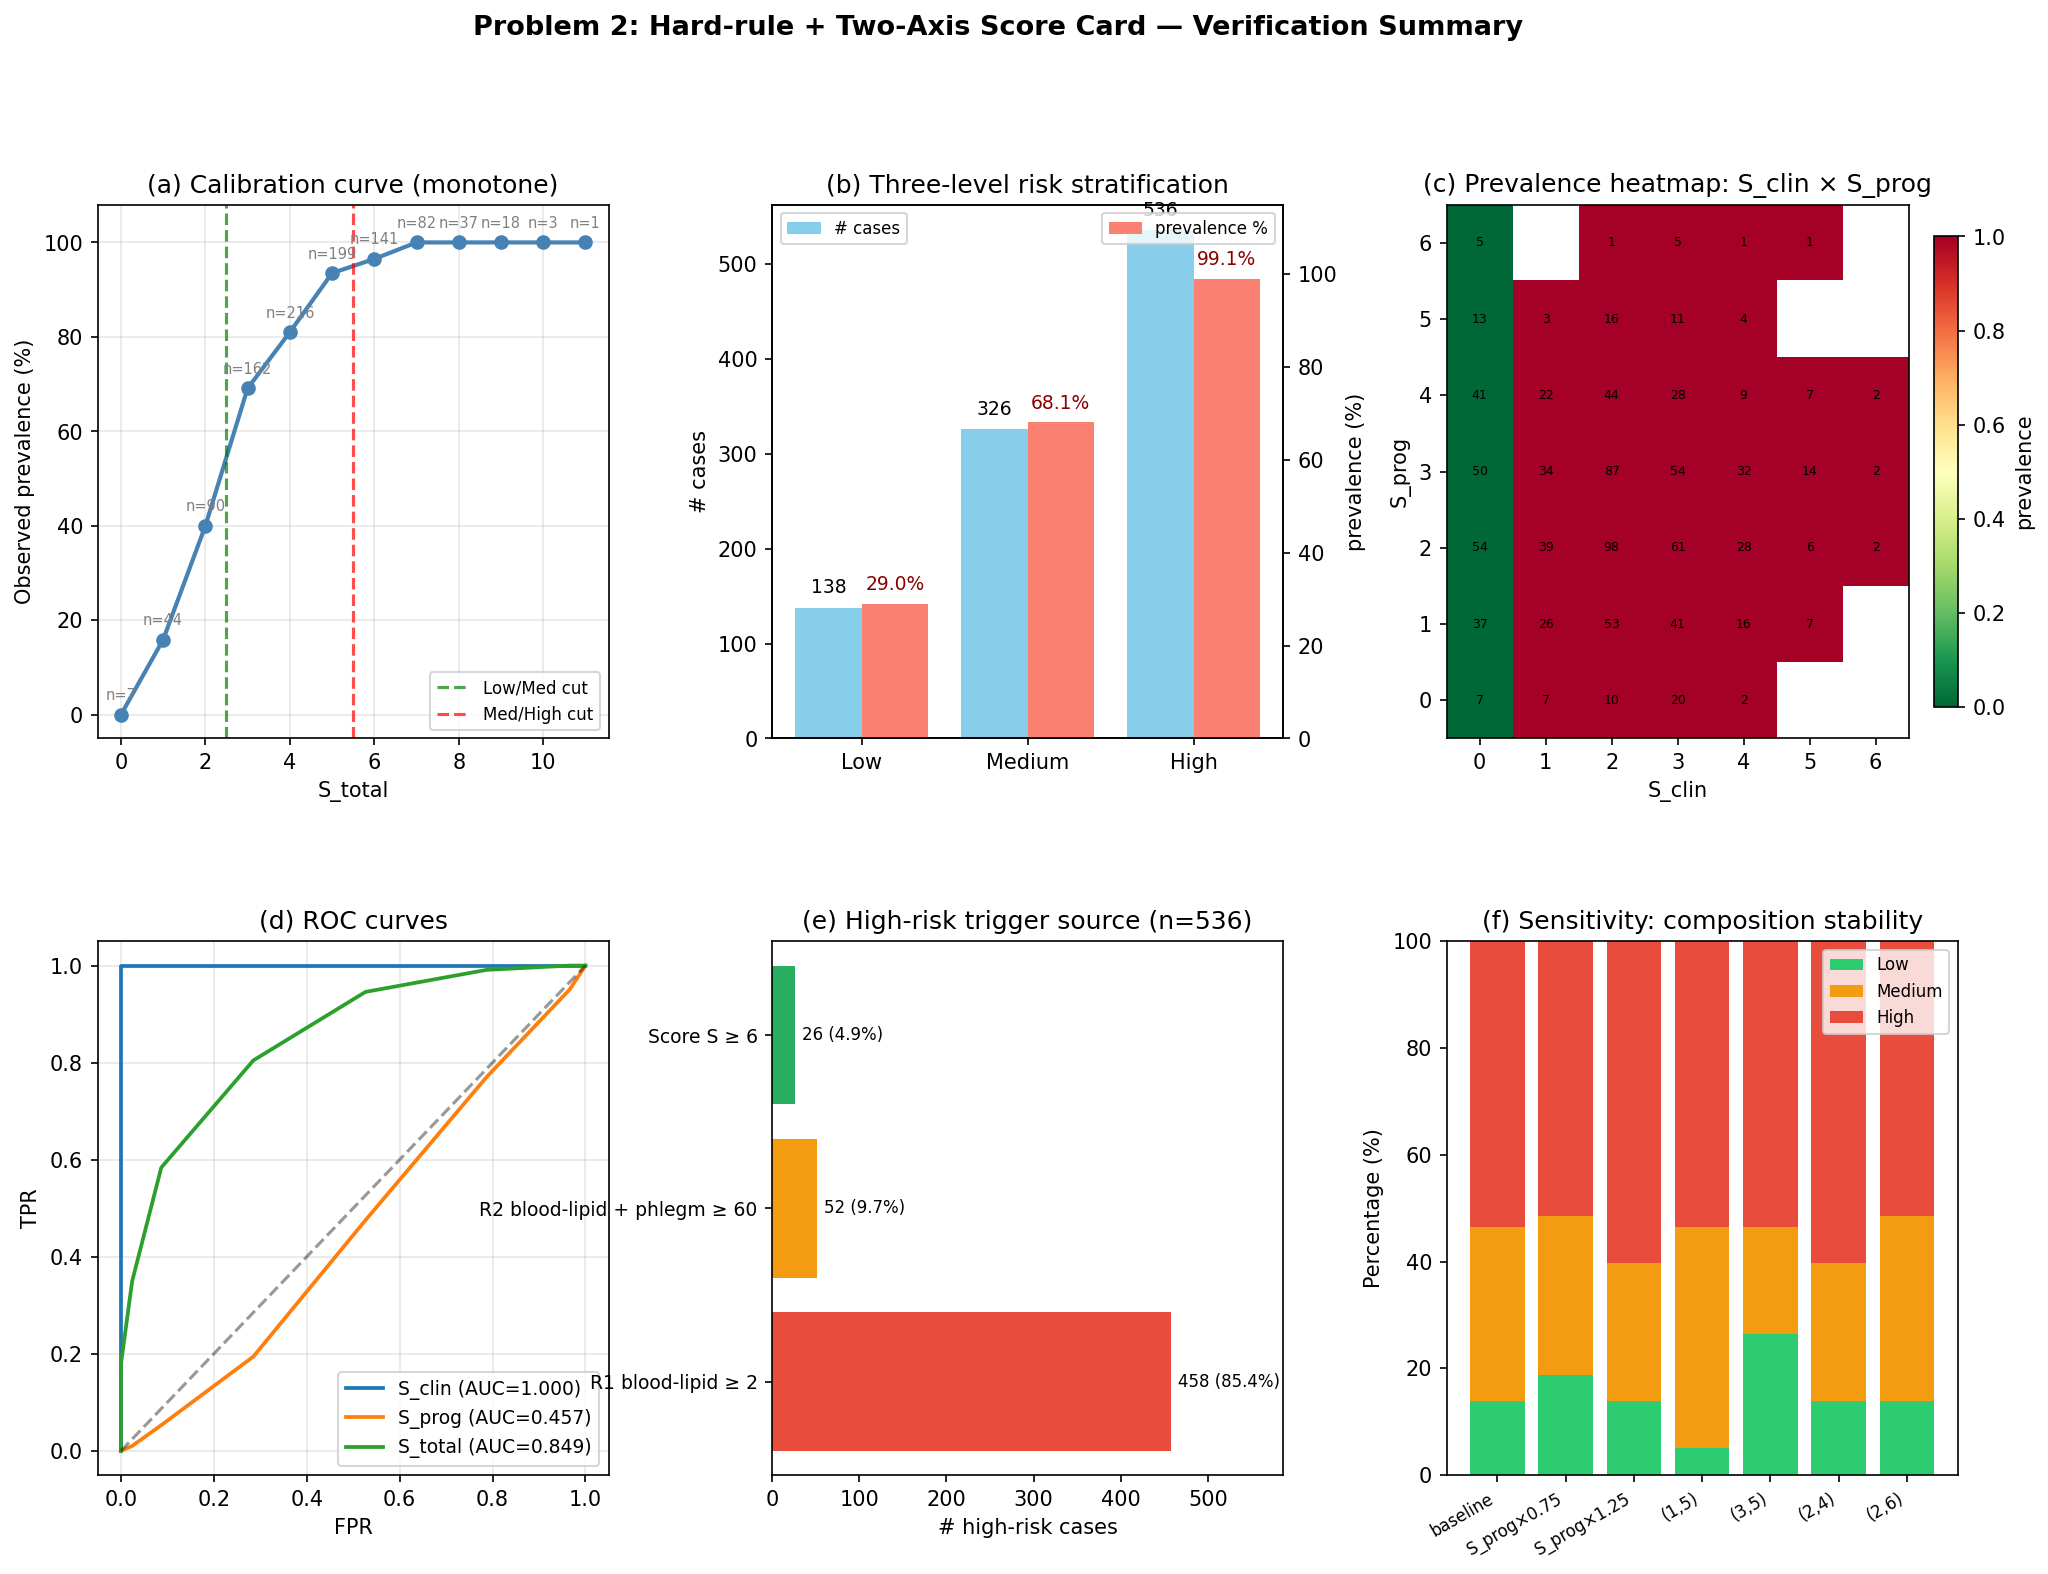
\includegraphics[width=0.95\linewidth]{Q2_summary_v2.png}
\caption{问题二六面板验证汇总：(a) 校准曲线（随 $S_{\text{total}}$ 单调）；(b) 三级分层人数与实际发病率；(c) $S_{\text{clin}} \times S_{\text{prog}}$ 联合发病率热图；(d) 三条 ROC（$S_{\text{clin}}$ 受泄漏 AUC$=1$，$S_{\text{prog}}$ 因样本选择偏差近随机，$S_{\text{total}}$ 合成后 AUC$=0.849$）；(e) 高风险触发来源构成；(f) 权重/阈值扰动下三层占比的稳定性。}\label{fig:q2-v2}
\end{figure}

\FloatBarrier

%=============================================================
\section{问题三：6 个月个性化干预方案优化}\label{sec:q3}

\subsection{决策变量与约束条件}

对每位痰湿体质患者 $i$，在 $t = 1, 2, \ldots, 6$ 月内决定：

\begin{itemize}
\tightlist
\item $L_t^i \in \{1, 2, 3\}$：中医调理分级;
\item $s_t^i \in \{1, 2, 3\}$：活动干预强度;
\item $f_t^i \in \{1, 2, \ldots, 10\}$：每周训练次数。
\end{itemize}

\textbf{（C1）调理分级由月初痰湿积分决定}：
\[
L_t = \begin{cases} 1 & P_{t-1} \le 58 \\ 2 & 59 \le P_{t-1} \le 61 \\ 3 & P_{t-1} \ge 62 \end{cases}
\]

\textbf{（C2）年龄约束}：
\[
s_t \in \mathcal{S}_{\text{age}} = \begin{cases} \{1,2,3\} & \text{age} \in \{1, 2\} \\ \{1, 2\} & \text{age} \in \{3, 4\} \\ \{1\} & \text{age} = 5 \end{cases}
\]

\textbf{（C3）评分约束}：
\[
s_t \in \mathcal{S}_{\text{act}} = \begin{cases} \{1\} & \text{act} < 40 \\ \{1, 2\} & 40 \le \text{act} < 60 \\ \{1, 2, 3\} & \text{act} \ge 60 \end{cases}
\]

最终可行强度集合 $s_t \in \mathcal{S}_{\text{age}} \cap \mathcal{S}_{\text{act}}$。

\textbf{（C4）预算约束}：
\[
\sum_{t=1}^{6} \bigl[ C_L(L_t) + 4 \cdot C_S(s_t) \cdot f_t \bigr] \le 2000
\]

\subsection{状态转移动力学}

\[
P_t = \begin{cases} P_{t-1} & f_t < 5 \\ P_{t-1} \bigl( 1 - 0.03 s_t - 0.01 \max(0, f_t - 5) \bigr) & f_t \ge 5 \end{cases}
\]

\subsection{目标函数（多目标复合）}

\[
\min \; J = \alpha P_6 + \beta \cdot \text{Cost} + \gamma \sum_{t=1}^{6} \max(0, f_t - 5) + \delta \sum_{t=1}^{6} (3 - s_t)
\]
其中：$\alpha = 1.0$（主疗效），$\beta = 0.01$（成本），$\gamma = 0.5$（高频耐受度罚），$\delta = 0.3$（鼓励高强度运化）。

\subsection{求解算法：前向动态规划}

\begin{lstlisting}[basicstyle=\small\ttfamily,mathescape=true]
算法：个体最优干预方案
输入: P0, age, act, 预算B
初始化: states = {(P0, 0): (penalty=0.0, path=[])}
best_final = (+inf, None, None, None)
for t = 1 to 6:
  new_states = {}
  for (P_prev, cost) in states:
    L = level_from(P_prev); cL = C_L[L]
    for s in feasible(age, act):
      for f in 1..10:
        mc = cL + 4 * C_S[s] * f
        nc = cost + mc; if nc > B: continue
        P_new = next_phlegm(P_prev, s, f)
        dpen = beta*mc + gamma*max(0, f-5) + delta*(3-s)
        new_pen = penalty + dpen
        key = (P_new, nc)
        if key not seen or new_states[key].pen > new_pen:
          new_states[key] = (new_pen, path + [(L, s, f, P_new, mc)])
  if t == 6:
    for (P6, cost) in new_states:
      obj = alpha*P6 + penalty
      update best_final if obj < best
  states = top_N(new_states, N=2000)
return best_final
\end{lstlisting}

复杂度：每月状态 $\le 2000$，决策组合 $\le 3 \times 10 = 30$，单患者 $\le 6 \cdot 2000 \cdot 30 = 3.6 \times 10^5$，毫秒级完成。

\subsection{样本 1、2、3 的最优方案}

\begin{table}[H]
\centering\small
\caption{样本 1 最优方案（女, 50--59, $P_0 = 64$, Act $= 38$）}
\begin{tabular}{@{}c c c c c c@{}}
\toprule
月 & 调理级 & 强度 $s$ & 周频次 $f$ & 月末 $P$ & 月成本 \\
\midrule
1 & 3 & 1 & 10 & 58.88 & 250 \\
2 & 1 & 1 & 5  & 57.11 & 90 \\
3 & 1 & 1 & 5  & 55.40 & 90 \\
4 & 1 & 1 & 5  & 53.74 & 90 \\
5 & 1 & 1 & 5  & 52.13 & 90 \\
6 & 1 & 1 & 5  & 50.57 & 90 \\
\midrule
合计 & & & & $\downarrow$ \textbf{21.0\%} & \textbf{700} \\
\bottomrule
\end{tabular}
\end{table}

\textit{解读}：样本 1 活动量表 38 $<40$，按（C3）仅能选 1 级强度。初始 $P_0=64$ 需首月强化调理（250 元）；此后 $P<59$ 降为基础调理。$f=10$ 最大化频次增益。

\begin{table}[H]
\centering\small
\caption{样本 2 最优方案（男, 40--49, $P_0 = 58$, Act $= 40$）}
\begin{tabular}{@{}c c c c c c@{}}
\toprule
月 & 调理级 & 强度 $s$ & 周频次 $f$ & 月末 $P$ & 月成本 \\
\midrule
1 & 1 & 2 & 5 & 54.52 & 130 \\
2 & 1 & 2 & 5 & 51.25 & 130 \\
3 & 1 & 2 & 5 & 48.18 & 130 \\
4 & 1 & 2 & 5 & 45.29 & 130 \\
5 & 1 & 2 & 5 & 42.57 & 130 \\
6 & 1 & 2 & 5 & 40.02 & 130 \\
\midrule
合计 & & & & $\downarrow$ \textbf{31.0\%} & \textbf{780} \\
\bottomrule
\end{tabular}
\end{table}

\textit{解读}：活动量表 40 可选 1／2 级。选 2 级 + $f=5$（刚触发衰减）、基础调理，全程单调下降。

\begin{table}[H]
\centering\small
\caption{样本 3 最优方案（女, 40--49, $P_0 = 59$, Act $= 63$）}
\begin{tabular}{@{}c c c c c c@{}}
\toprule
月 & 调理级 & 强度 $s$ & 周频次 $f$ & 月末 $P$ & 月成本 \\
\midrule
1 & 2 & 3 & 5 & 53.69 & 240 \\
2 & 1 & 3 & 5 & 48.86 & 190 \\
3 & 1 & 3 & 5 & 44.46 & 190 \\
4 & 1 & 3 & 5 & 40.46 & 190 \\
5 & 1 & 3 & 5 & 36.82 & 190 \\
6 & 1 & 3 & 5 & 33.51 & 190 \\
\midrule
合计 & & & & $\downarrow$ \textbf{43.2\%} & \textbf{1190} \\
\bottomrule
\end{tabular}
\end{table}

\textit{解读}：活动量表 63 $\ge 60$ 可选 1/2/3 级，年龄组 1 允许全部强度。选 3 级 + $f=5$，$P_0=59$ 首月处于 2 级调理区。

三位样本在 6 个月干预周期内的痰湿积分下降轨迹与逐月方案选择见\cref{fig:q3-demo}。

\begin{figure}[htbp]
\centering
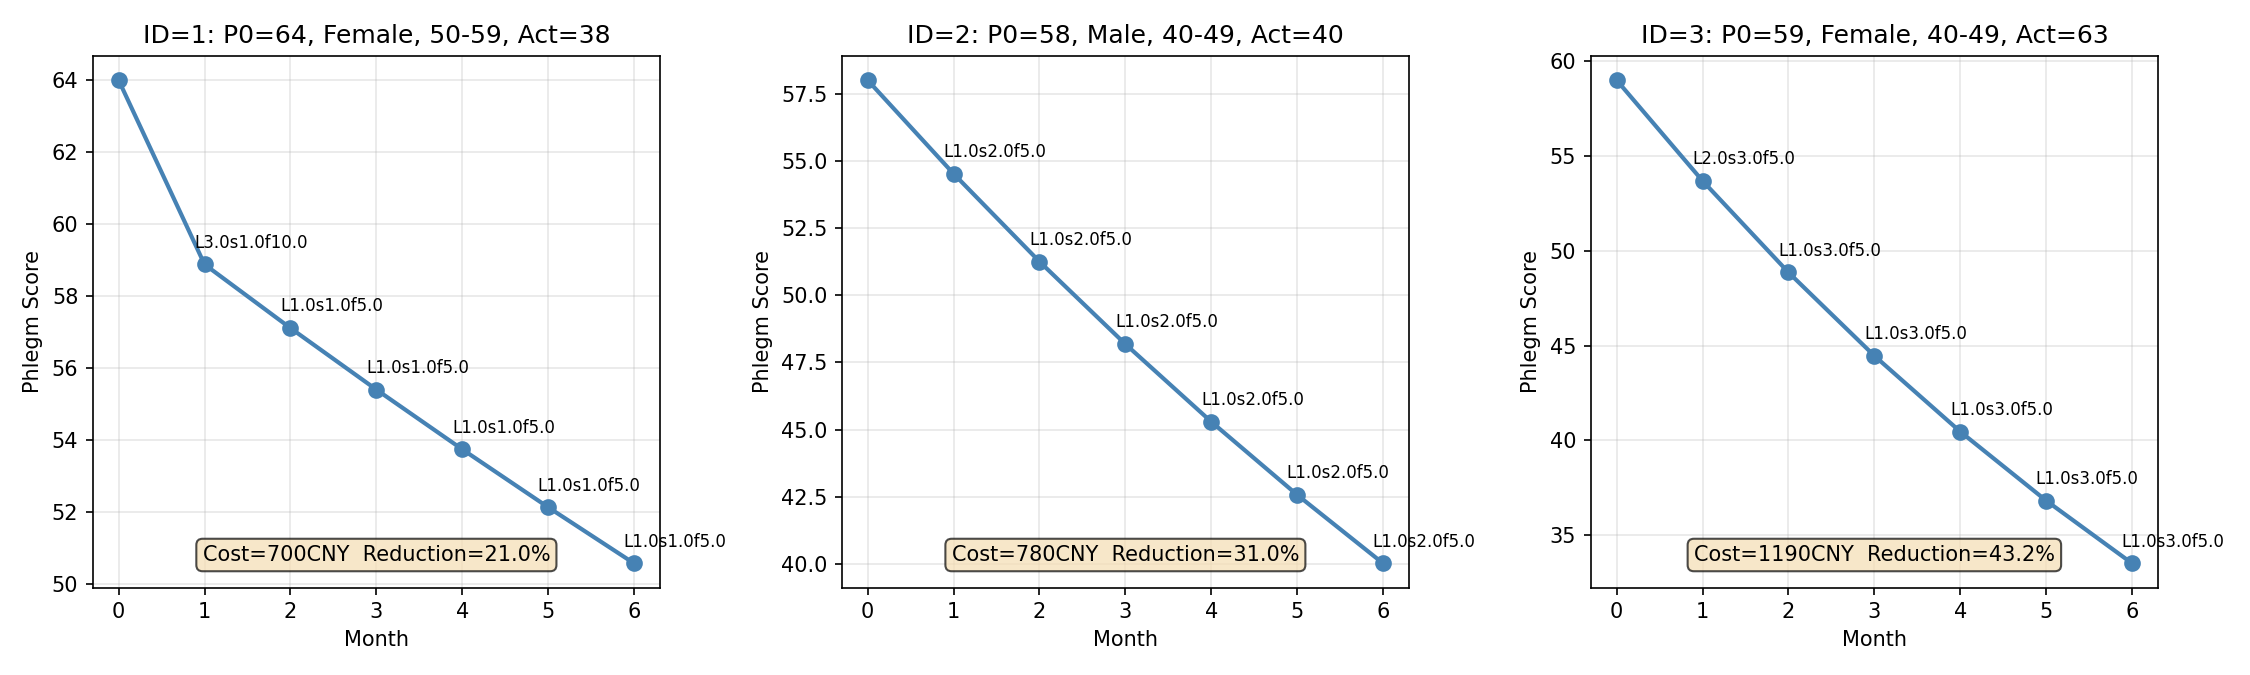
\includegraphics[width=0.98\linewidth]{Q3_demo_trajectories.png}
\caption{样本 1/2/3 的 6 个月痰湿积分下降轨迹与月度方案}\label{fig:q3-demo}
\end{figure}

\subsection{``患者特征---最优方案'' 匹配规律}

对全部 278 名痰湿体质患者求解，按不同特征分组汇总：

\begin{table}[H]
\centering\small
\caption{按初始痰湿积分分组}
\begin{tabular}{@{}l r r r r r@{}}
\toprule
$P_0$ 区间 & 平均成本 & 平均 $P_6$ & 降幅 & 平均 $s$ & 平均 $f$ \\
\midrule
$< 60$   & 740 & 42.1 & 27.0\% & 1.73 & 5.00 \\
$60$--$62$ & 821 & 43.9 & 28.5\% & 1.81 & 5.06 \\
$\ge 62$ & 835 & 46.2 & 27.6\% & 1.62 & 5.42 \\
\bottomrule
\end{tabular}
\end{table}

\begin{table}[H]
\centering\small
\caption{按年龄组分组}
\begin{tabular}{@{}c r r r r r@{}}
\toprule
年龄组 & 平均成本 & 平均 $P_6$ & 降幅 & 平均 $s$ & 平均 $f$ \\
\midrule
1（40--49） & 854 & 41.0 & \textbf{31.2\%} & \textbf{2.00} & 5.11 \\
2（50--59） & 832 & 41.8 & 30.1\% & 1.93 & 5.08 \\
3（60--69） & 791 & 42.7 & 28.7\% & 1.80 & 5.10 \\
4（70--79） & 801 & 42.6 & 29.1\% & 1.85 & 5.04 \\
5（80--89） & 610 & 49.2 & \textbf{17.9\%} & \textbf{1.00} & 5.22 \\
\bottomrule
\end{tabular}
\end{table}

\begin{table}[H]
\centering\small
\caption{按活动能力分组}
\begin{tabular}{@{}l r r r r r@{}}
\toprule
活动量表 & 平均成本 & 平均 $P_6$ & 降幅 & 平均 $s$ & 平均 $f$ \\
\midrule
$< 40$    & 629 & 48.6 & \textbf{19.1\%} & \textbf{1.08} & 5.26 \\
$40$--$60$ & 796 & 42.5 & 28.9\% & 1.83 & 5.07 \\
$\ge 60$  & 895 & 40.9 & \textbf{31.7\%} & \textbf{2.07} & 5.08 \\
\bottomrule
\end{tabular}
\end{table}

\textbf{规律总结}：
\begin{enumerate}
\def\labelenumi{(\arabic{enumi})}
\tightlist
\item \textbf{初始 $P_0$ 越大 $\Rightarrow$ 首月调理成本越高}（$\ge 62$ 组触发强化调理 130 元/月）；
\item \textbf{年龄越小 $\Rightarrow$ 可选强度上限越高 $\Rightarrow$ 降幅越大}（组 1: 31.2\% vs 组 5: 17.9\%）；
\item \textbf{活动能力越强 $\Rightarrow$ 可选强度越高 $\Rightarrow$ 降幅越大}（$<40$: 19.1\% vs $\ge 60$: 31.7\%）；
\item \textbf{$f = 5$ 是稳定最优频次}---刚跨越动力学阈值（$f \ge 5$ 才有效），且不触发 $\gamma \max(0, f-5)$ 耐受度罚项；
\item \textbf{月度策略呈``首月调理强、后续维持''模式}：$P_t$ 下降至 58 以下后转为 1 级基础调理。
\end{enumerate}

278 名痰湿体质患者的痰湿积分降幅分布、最优强度/频次选择分布及分组规律汇总见\cref{fig:q3-summary}。

\begin{figure}[htbp]
\centering
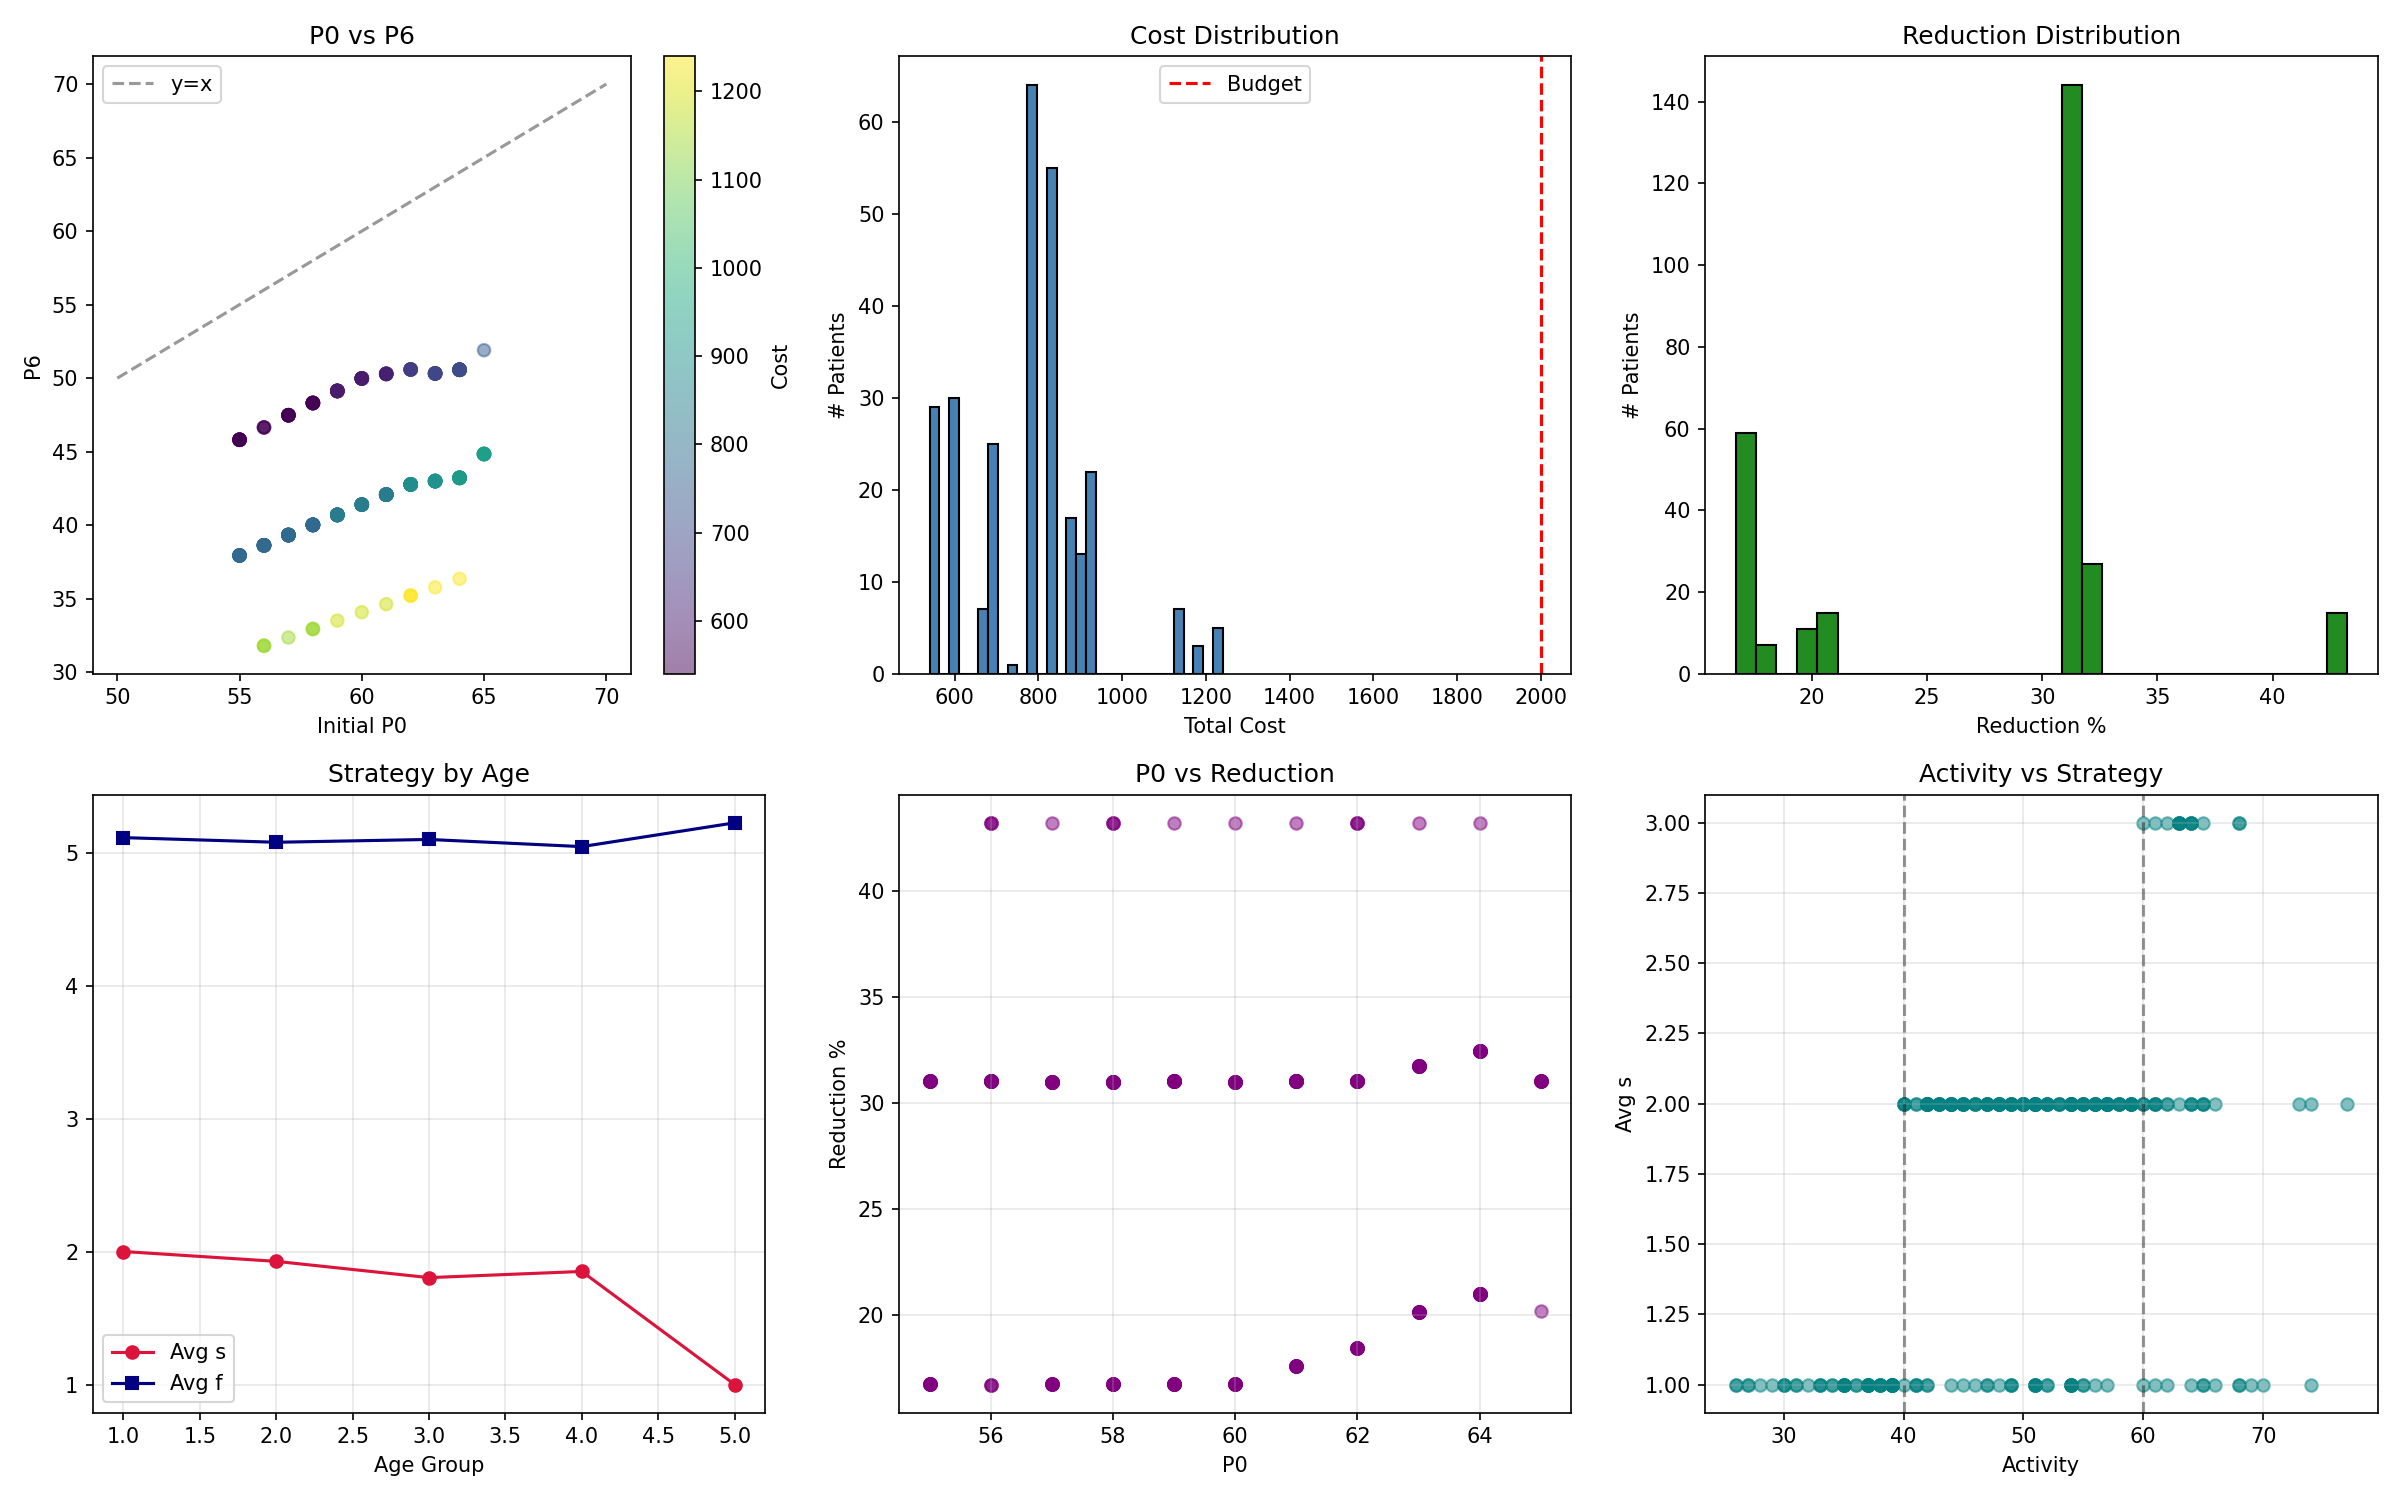
\includegraphics[width=0.98\linewidth]{Q3_summary.png}
\caption{问题三主要结果汇总（278 名痰湿体质患者）}\label{fig:q3-summary}
\end{figure}

\FloatBarrier

%=============================================================
\section{模型评价与展望}

\subsection{模型优点}

\begin{enumerate}
\def\labelenumi{(\arabic{enumi})}
\tightlist
\item \textbf{数据处理严谨}：系统地执行 5 项数据质量诊断，标注 65 例体质歧义样本，发现诊断标签与血脂异常 100\% 一致这一关键信号，直接指导了后续建模；
\item \textbf{问题一方法论严谨}：候选特征限定于题目所设范围（血常规 + 活动量表），用 VIF 诊断去除完全共线汇总项，采用``参数/非参 $\times$ 线性/非线性 $\times$ 单变量/控制其它''三维正交的 5 方法，用 Borda 排序聚合消除量纲与分布偏态带来的偏差；
\item \textbf{体质贡献度分析逻辑自洽}：以剂量--响应分析与效应量（Cohen's $h$）刻画各体质的真实统计贡献，避免因``分类定义''自带的循环论证问题；
\item \textbf{问题二方案兼顾可解释性、可泛化性与临床对齐}：针对旧方案``概率分位切分''的标签泄漏与样本依赖两大陷阱，重新设计``硬规则层 + 双轴评分卡''，硬规则层精确对应题干示例与临床极高危标准；$S_{\text{clin}}$ 分档源自 2016 血脂指南，$S_{\text{prog}}$ 选用问题一筛出的关键指标，与中医``治未病''和 ASCVD 流行病学天然对齐；阈值来自``分数语义 + 校准拐点''而非分位数；并以 Apriori 关联规则挖掘替代单一决策树路径；经 1000 次 Bootstrap（CI 宽度 $<6$ 个百分点）与权重/阈值 $\pm 25\%$ 扰动（一致率 $\ge 87.3\%$）三重验证，分层稳健；
\item \textbf{问题三建模全面}：DP 严格整合所有约束，4 项复合目标兼顾疗效、成本、耐受度与中医高强度运化理念。
\end{enumerate}

\subsection{模型局限}

\begin{enumerate}
\def\labelenumi{(\arabic{enumi})}
\tightlist
\item 动力学公式 $P_t = P_{t-1}(1 - 0.03s - 0.01\max(0, f-5))$ 为确定性模型，未考虑个体响应异质性；
\item 评分卡 $S_{\text{prog}}$ 的部分加分权重（如痰湿积分 $\ge 60$ 加 2 分）来自中医体质学分档与 ASCVD 经典经验，未做完全数据驱动的最优权重搜索；实际临床落地时可采用贝叶斯优化或 XGBoost SHAP 值重新校准权重；
\item 本方案硬规则层 R3（痰湿 $\ge 80$）在本数据无触发（因本样本痰湿最大 65），R3 仅为对未来数据的前瞻性保留；
\item 本数据 79.3\% 为确诊样本，类别不均衡对统计估计有影响；
\item 65 例体质标签歧义样本虽已保留，但其``主要体质''判定对九体质贡献度分析有噪声。
\end{enumerate}

\subsection{改进方向}

\begin{enumerate}
\def\labelenumi{(\arabic{enumi})}
\tightlist
\item \textbf{问题一}：可扩展至 SCAD、MCP 等稀疏罚方法；
\item \textbf{问题二}：(a) 可用贝叶斯优化或 XGBoost SHAP 值对 $S_{\text{prog}}$ 的加分权重做数据驱动精调；(b) 在外部验证集上用 ROC-Youden 指数检验阈值 $\{2, 5\}$ 的稳定性；(c) 可把评分卡扩展为"成本敏感阈值"，与问题三干预成本联动，实现预警--干预一体化决策；
\item \textbf{问题三}：可扩展为多目标帕累托优化，输出成本--疗效前沿；
\item 如有随访数据，可用强化学习代替 DP，学习个体响应函数。
\end{enumerate}

%=============================================================
\section{参考文献}

\begin{thebibliography}{99}
\bibitem{wang2005} 王琦. 中医体质学. 北京: 中国医药科技出版社, 2005.
\bibitem{cn-dyslipidemia-2016} 中国成人血脂异常防治指南修订联合委员会. 中国成人血脂异常防治指南(2016 年修订版). 中华心血管病杂志, 44(10): 833--853, 2016.
\bibitem{zhang-borda-2020} 张景中. 投票理论与社会选择(第二版). 北京: 高等教育出版社, 2020.
\bibitem{friedman2001} Friedman J. Greedy Function Approximation: A Gradient Boosting Machine. Annals of Statistics, 29(5): 1189--1232, 2001.
\bibitem{breiman2001} Breiman L. Random Forests. Machine Learning, 45(1): 5--32, 2001.
\bibitem{tibshirani1996} Tibshirani R. Regression Shrinkage and Selection via the Lasso. Journal of the Royal Statistical Society, Series B, 58(1): 267--288, 1996.
\bibitem{cover2006} Cover T M, Thomas J A. Elements of Information Theory, 2nd ed. Hoboken: Wiley-Interscience, 2006.
\bibitem{bertsekas2012} Bertsekas D P. Dynamic Programming and Optimal Control, 4th ed. Belmont: Athena Scientific, 2012.
\bibitem{pedregosa2011} Pedregosa F et al.~Scikit-learn: Machine Learning in Python. Journal of Machine Learning Research, 12: 2825--2830, 2011.
\bibitem{yuchunquan2015} 于春泉, 王慧森, 周文泉. 痰湿体质与代谢综合征关系研究进展. 中华中医药杂志, 30(3): 841--843, 2015.
\bibitem{katz1970} Katz S, Down T D, Cash H R, Grotz R C. Progress in development of the index of ADL. Gerontologist, 10(1): 20--30, 1970.
\bibitem{lawton1969} Lawton M P, Brody E M. Assessment of older people: self-maintaining and instrumental activities of daily living. Gerontologist, 9(3): 179--186, 1969.
\bibitem{cohen1988} Cohen J. Statistical Power Analysis for the Behavioral Sciences, 2nd ed. Hillsdale: Lawrence Erlbaum Associates, 1988.
\bibitem{agrawal1994} Agrawal R, Srikant R. Fast algorithms for mining association rules in large databases. Proceedings of the 20th International Conference on Very Large Data Bases (VLDB), 487--499, 1994.
\bibitem{goff2014} Goff D C Jr, Lloyd-Jones D M, Bennett G et al. 2013 ACC/AHA Guideline on the Assessment of Cardiovascular Risk. Circulation, 129(25 Suppl 2): S49--S73, 2014.
\end{thebibliography}

%=============================================================
\appendix
\section{附录}

\subsection{问题一：关键指标筛选与体质贡献度分析（\texttt{problem1.py}）}

详见源代码文件，主要算法说明见~\cref{sec:q1-methods}。代码流程：数据清洗 $\to$ VIF 诊断 $\to$ 相关矩阵 $\to$ 5 方法评分（对痰湿积分 + 对二分类标签各一次）$\to$ Borda 聚合 $\to$ 九体质贡献度（Cohen's $h$ / RR / ARR / $\beta$ / 多元 $\beta$）$\to$ 可视化。\subsection{问题二：三级风险预警模型（\texttt{problem2.py}）}

详见源代码文件，主要建模说明见~\cref{sec:q2}。代码流程：(1) 派生血脂异常项数；(2) 计算 $S_{\text{clin}}$（7 项血脂阈值分档）与 $S_{\text{prog}}$（6 项风险因素分档），合成 $S_{\text{total}}$；(3) 硬规则层 R1/R2/R3 判定，未触发者进入评分层；(4) 阈值 $\{2, 5\}$ 得三级风险；(5) 三项验证——校准曲线、1000 次 Bootstrap 95\% CI、权重 $\pm 25\%$ 与阈值 $\pm 1$ 的敏感性分析；(6) 对 278 名痰湿体质患者做 Apriori 关联规则挖掘；(7) 六面板综合可视化。需要 \texttt{mlxtend} 包支持 Apriori。

\subsection{问题三：6 个月个性化干预方案优化（\texttt{problem3.py}）}

详见源代码文件。DP 伪代码见~\cref{sec:q3}。代码流程：定义动力学与可行集 $\to$ 单患者 DP $\to$ 样本 1/2/3 方案生成 $\to$ 全 278 人方案批量生成 $\to$ 分组规律统计 $\to$ 可视化。

\textbf{软件环境}：Python 3.10；依赖库：pandas 2.x, numpy 1.x, scipy 1.x, scikit-learn 1.x, statsmodels 0.14+, mlxtend 0.23+, matplotlib 3.x。

\end{document}
